\documentclass[10pt, a4paper]{report}

%\usepackage{fancyhdr}
\usepackage{hyperref}
\usepackage[T1]{fontenc}
\usepackage{ae,aecompl}
\usepackage{graphicx}
\usepackage[left=2cm, right=2cm, top=3cm, bottom=2.5cm]{geometry}
\usepackage{latexsym}
\usepackage{amsmath, amsthm, amssymb}
\usepackage{rotating}
\usepackage{boxedminipage}
\usepackage{multicol}

% Package for including code in the document
\usepackage{listings}

% If you want to generate a toc for each chapter (use with book)
% \usepackage{minitoc}

\begin{titlepage}
\title{Calcolo Numerico} 
\author{Massimo Nocentini}
\end{titlepage}
% My Theorem
\newtheorem{oss}{Osservation}[section]
\newtheorem{exercise}{Exercise}[section]
\newtheorem{thm}{Theorem}[section]
\newtheorem{cor}[thm]{Corollary}
\newtheorem{lem}[thm]{Lemma}

\newcommand{\vect}[1]{\boldsymbol{#1}}
% instead of boldsymbol I can use the arrow above the letter with
%\newcommand{\vect}[1]{\vec{#1}}

% page settings
\pagestyle{headings}

\begin{document}

% settings for the lstlisting environment
\lstset{
	language = octave
	, numbers = left 
	, basicstyle=\sffamily%\footnotesize
	, frame=single
	, tabsize=2
	, captionpos=b
	, breaklines=true
	, showspaces=false
	, showstringspaces=false
}

\maketitle

\tableofcontents

\newpage

\section*{Introduzione}
Queste note contengono tutto il mio materiale di studio per l'esame di Calcolo Numerico.

\subsection*{Sintassi esercizi}
Per gli esercizi utilizzo questa sintassi \textbf{Exercise n[(m)]}, dove $n$
rappresenta la numerazione locale all'interno delle sezioni di questo documento, 
$m$ rappresenta l'identificativo dell'esercizio fissato nel libro di testo 
\textbf{Calcolo Numerico} di \emph{Brugnano, Magherini, Sestini} pubblicato da \emph{Master}, 
prima edizione.
Il reference $(m)$ non \`e sempre presente, come evidenziato dall'uso delle parentesi quadre.



\chapter{Errori ed aritmetica finita}

\section{Discretizzazione} 

Questi errori sorgono tutte le volte che si vuole modellare un problema 
matematico (formulato nel continuo) con un sistema discreto. Per ottenere 
questo, uso dei processi di discretizzazione, dei quali mi interessa controllare
quanto ``bene'' approssimano il problema che voglio modellare.

Pi\`u specificamente, l'errore di troncamento \emph{locale} corrisponde 
all'errore introdotto nel passo di integrazione corrente assumendo esatto il 
valore di partenza, mentre l'errore di troncamento \emph{globale} rappresenta 
l'effetto di tutti gli errori precedenti.

Per i seguenti due esercizi si utilizza la formula di Taylor-Peano, con il 
resto ''infinitesimo di ordine superiore'' rispetto al massimo grado $n$ a cui 
si arresta lo sviluppo e quindi consente di ottenere una approssimazione
locale, cio\`e in un intorno di $x_{0}$.

\begin{exercise}[1.1]
	Sia $x = \pi \approx 3.14159265$. Considero come valore approssimato 
	$\tilde{x} = 3.1415$. 
	
	Calcolare il corrispondente errore relativo\footnote{D\'a l'ordine di 
	grandezza rispetto alla base $10$} $\varepsilon_{x}$. 
	
	Verificare che il numero di cifre decimali corrette nella rappresentazione 
	approssimata di $x$ mediante $\tilde{x}$ all'incirca \`e dato da $-\log_{10}
	{|\varepsilon_{x}|}$.
\end{exercise}
Ottengo:
\begin{displaymath}
	\varepsilon_{x} = \frac{\tilde{x}-x}{x} = \frac{3.1415-3.14159265358979}
	{3.14159265358979}
\end{displaymath}
\begin{lstlisting}
octave:19> (3.1415-pi)/pi
ans = -2.94925536215087e-05
\end{lstlisting}
Adesso considero:
\begin{equation*}
	-\log_{10}{|-2.9491 \times 10^{-5}|} = -\left (\log_{10}{2.9491} +
	\log_{10}{10^{-5}} \right ) = -\log_{10}{2.9491} + 5\log_{10}{10}
\end{equation*}
\begin{lstlisting}
octave:18> -log10(2.9491) + 5*log10(10)
ans =  4.53031050085890e+00
\end{lstlisting}
L'approssimazione $\tilde{x}$ ha 4 cifre decimali corrette.

\begin{exercise}
Dimostrare che $-\log_{10}{|\varepsilon_{x}|}$ d\`a all'incirca il numero 
di cifre decimali corrette di $\tilde{x}$, con cui approssimo $x$. 
\end{exercise}
\begin{proof}
Sia $r$ il numero di cifre decimali \emph{esatte}, tale che 
$r = -\log_{10}{|\varepsilon_{x}|}$. Passando agli esponenti ottengo 
$|\varepsilon_{x}| = 10^{-r}$.

Dato che cerco un'approssimazione del numero di cifre decimali a partire dall'
errore relativo, imposto due disequazioni per trovare un intervallo in cui $r$
pu\`o variare.

Scrivo in forma normalizzata il valore esatto $x$ e la sua approssimazione 
$\tilde{x}$, fissando $\beta = 10$ e $M \not = m$ perch\`e sto approssimando:
\begin{equation*}
	\begin{split}
		x \in \mathbb{R}, x \geq 0, x = m \times 10^{e} \\
		\tilde{x} \in \mathbb{R}, \tilde{x} \geq 0, \tilde{x} = M \times 10^{e}
	\end{split}
\end{equation*}
Per il \emph{teorema 1.2} vale $ 1 \leq m < 10 \wedge  1 \leq M < 10$.

Adesso voglio trovare sia una maggiorazione che una minorazione di 
$\varepsilon_{x}$:
\begin{equation*}
	\left | \varepsilon_{x} \right | = \left | \frac{(M - m) \times 10^{e}} 
		{m \times 10^{e}}
	\right | = \left | \frac{M - m}{m} \right |
\end{equation*}
Maggioro con:
\begin{equation*}
	\left | \frac{M - m}{m} \right | < 10 = max
\end{equation*}
In quanto il massimo lo ottengo quando $M = 9, m = 1$.

Minoro con:
\begin{equation*}
	min = \frac{1}{10} \le \left | \frac{M - m}{m} \right | 
\end{equation*}
In quanto il minimo lo ottengo quando $M = 8, m = 9$.

Adesso posso impostare le due disequazioni:
\begin{equation*}
	10^{-r -1} = \frac{\left | \varepsilon_{x} \right |}{10} \le 
		\left | \varepsilon_{x} \right | <
	10 \left | \varepsilon_{x} \right | = 10^{-r +1}
\end{equation*}
Le uguaglianze esterne valgono per quanto detto ad inizio prova.
%10^{-r-1} \leq |\varepsilon_{x}| < 10^{-r+1}
Passo ai logaritmi:
\begin{equation*}
	\begin{split}
		-r-1 \leq  \log_{10}{|\varepsilon_{x}|} < -r+1 \\
		r+1 \geq -\log_{10}{|\varepsilon_{x}|} > r-1
	\end{split}
\end{equation*}
Considero i rami $-r-1 \leq  \log_{10}{|\varepsilon_{x}|}$ dalla prima e 
$-\log_{10}{|\varepsilon_{x}|} > r-1$ dalla seconda per avere l'intervallo di variazione di $r$:
\begin{equation*}
	-1 - \log_{10}{|\varepsilon_{x}|} \leq r < 1 - \log_{10}{|\varepsilon_{x}|}
\end{equation*}
\end{proof}

\begin{exercise}[1.2]
	Dimostrare che, se $f(x)$ \`e sufficientemente regolare e $h>0$ \`e una 
	quantit\`a piccola, allora:
	\begin{equation*}
		\begin{split}
			\frac{f(x_{0}+h) - f(x_{0}-h)}{2h} =& f'(x_{0}) + O(h^{2}), \\
			\frac{f(x_{0}+h) - 2f(x_{0}) + f(x_{0}-h)}{h^{2}} =& f''(x_{0}) + O(h^{2}) 
		\end{split}
	\end{equation*}
\end{exercise}
Per entrambe considero gli sviluppi di Taylor di $f(x_{0}+h)$ e $f(x_{0}-h)$ in
$x_{0}$:
\begin{equation*}
	\begin{split}
		T(x_{0} + h)& = f(x_{0}) + f'(x_{0})h + \frac{f''(x_{0})h^{2}}{2} + 
		\frac{f'''(x_{0})h^{3}}{6} + O(h^{4}) \\ 
		T(x_{0} - h)& = f(x_{0}) - f'(x_{0})h + \frac{f''(x_{0})h^{2}}{2} - 
		\frac{f'''(x_{0})h^{3}}{6} + O(h^{4})
	\end{split}
\end{equation*}
Devo prestare attenzione al segno di alcuni termini dello sviluppo
\footnote{Attenzione: nello sviluppo di Taylor di una funzione $f(x)$,  le
derivate $n$-esime vengono calcolate nel punto $x_{0}$ in cui si vuole 
centrare lo sviluppo, e non nell'argomento della funzione}:
\begin{itemize}
	\item nel primo sviluppo, la combinazione lineare ammette tutti segni 
	positivi in quanto il passo di discretizzazione \`e positivo, ovvero si cerca
	di approssimare con valori $ > x_{0}$.
	\item nel secondo invece, il fattore $((x_{0} - h - x_{0} =h))^{k} < 0, 
	\forall{k=2n+1, n \in \mathbb{N}}$ fa si che i termini dello sviluppo di 
	grado dispari siano negativi, in quanto si sta discretizzando con un valore 
	minore a $x_{0}$, di conseguenza $x - x_{0} < 0$.
\end{itemize}
Sottraendo termine a termine e semplificando dove possibile ottengo la prima equazione: 
\begin{equation*}
	T(x_{0}+h) - T(x_{0}-h) = 2f'(x_{0})h + \frac{f'''(x_{0})h^{3}}{3} + O(h^{4}) 
\end{equation*}
dividendo per $2h$: 
\begin{equation*}
	\frac{T(x_{0}+h) - T(x_{0}-h)}{2h} = f'(x_{0}) + \frac{f'''(x_{0})h^{2}}{3}  +
	O(h^{3})
\end{equation*}
Osserviamo che, per $h \rightarrow 0$, la quantit\`a $O(h^{3})$ diminuisce pi\`u 
velocemente del termine $$\frac{f'''(x_{0})h^{2}}{3}$$ per cui possiamo dedurre
che si approssima la derivata prima con una quantit\`a $O(h^{2})$.

Per la seconda equazione invece che sottrarre termine a termine, sommiamo,
ottenendo:
\begin{equation*}
	\begin{split}
		T(x_{0}+h) + T(x_{0}-h) = 2f(x_{0}) + f''(x_{0})h^{2} + O(h^{4})\\
		\frac{T(x_{0}+h) - 2f(x_{0}) + T(x_{0}-h)}{h^{2}} = f''(x_{0}) + O(h^{2}) 
	\end{split}
\end{equation*}
ovvero la quantit\`a al primo membro approssima la $f''(x_{0})$ con un errore 
dell'ordine $O(h^{2})$.

\section{Errori di convergenza}

\begin{exercise}[1.3] 
\label{exercise:exerciseIterativeMethodFixedPoint}
Dimostrare che il metodo iterativo $$x_{n+1}=\phi(x_{n})$$ convergente a x*,
deve verificare la condizione di \textbf{consistenza} $$x^{*}=\phi(x^{*})$$
ovvero la soluzione cercata deve essere un punto fisso per la funzione di
iterazione che definisce il metodo.
\end{exercise}
\begin{proof}
Suppongo che il metodo $\phi$ sia monotono e convergente a $x^{*}$. Definisco
il preordine $\rightarrow$ per catturare la convergenza:
\begin{displaymath}
\rightarrow = \lbrace (x_{n}, x_{n+1}) : x_{n+1} = \phi(x_{n}) \wedge \lim_{n
\rightarrow \infty}{x_{n}} = x^{*}
\rbrace
\end{displaymath}
Suppongo \emph{per assurdo} che $$\phi(x^{*}) = x^{\triangle} \not = x^{*}$$
Per l' ipotesi $x_{n} \rightarrow x^{*}$ (per la transitivit\`a di
$\rightarrow$), posso applicare la monotonia di $\phi$ rispetto a $\rightarrow$:
$$\phi(x_{n}) \rightarrow \phi(x^{*}) = x^{\triangle}$$ ma questo contraddice 
l'ipotesi che $\phi$ converge a $x^{*}$.
\end{proof}

\begin{exercise}
Considerare il metodo iterativo:
\begin{displaymath}
	x_{n+1} = \phi(x_{n}) = \frac{1}{2} \left ( x_{n} + \frac{2}{x_{n}} \right ), 
		\quad x_{0} = 2
\end{displaymath}
dimostrare che il metodo genera una successione di approssimazioni tale che 
$x_{n} \rightarrow \sqrt{2}$.
\end{exercise}
\begin{proof}
Questo metodo \`e a passo \emph{singolo} in quanto usa un solo innesto per calcolare
$x_{n + 1}$.
Affinch\`e il metodo iterativo sia convergente, per l'esercizio 
\ref{exercise:exerciseIterativeMethodFixedPoint} posso costruire
un'equazione per trovare il punto fisso di $\phi$:
\begin{displaymath}
\phi(x) = \frac{1}{2} \left ( x + \frac{2}{x} \right ) = x
\end{displaymath}
Manipolando: $x + \frac{2}{x} = 2x \Rightarrow x^{2} + 2 = 2x^{2} \Rightarrow 
	2 = x^{2}$
\end{proof}

\begin{exercise}[1.4] Per il testo dell'esercizio consultare il libro di testo.
\end{exercise}
Eseguendo il codice riportato nella sezione \nameref{sec:iterativeMethodToSQRT2}, 
questo \`e l'output di Octave sulla mia macchina:
\begin{lstlisting}
octave:8> iterative(2, 1.5)
next =  1.42857142857143e+00
Difference with last step:0.0714285714285714
next =  1.41463414634146e+00
Difference with last step:0.0139372822299655
next =  1.41421568627451e+00
Difference with last step:0.000418460066953008
next =  1.41421356268887e+00
Difference with last step:2.12358564088966e-06
next =  1.41421356237310e+00
Difference with last step:3.15774073555986e-10
Difference with sqrt(2):0
\end{lstlisting}
In 5 passi si raggiunge la precisione richiesta, uno in pi\`u rispetto ai risultati
mostrati in \emph{Tabella 1.1} del libro.




\section{Errori di round-off}
\section{Consigli per operazioni di macchina}
La seguente lista porta dei cosigli su come eseguire le operazioni di macchina a
quando si deve implementare un problema formulato in aritmetica esatta.

\begin{enumerate}
\item \emph{good approximation plus a small correction term} ecco alcuni
esempi
\begin{displaymath}
\begin{split}
a + \frac{b - a}{2} \quad & \text{\`e migliore di} \quad \frac{a + b}{2} \quad
\text{hint: } a - \frac{a}{2} = \frac{a}{2} \\ 
x - \frac{x^{2} - a}{2x} \quad & \text{\`e migliore di} \quad \frac{1}{2}\left
(x + \frac{a}{x} \right ) \quad \text{hint: } x - \frac{x}{2} = \frac{x}{2} \\
x_{2} - y_{2} \frac{x_{2} - x_{1}}{y_{2} - y_{1}} \quad & \text{\`e migliore di}
\quad \frac{y_{2}x_{1} - x_{2}y_{1}}{y_{2} - y_{1}} \quad
\text{hint: add } x_{2} - x_{2} \text{ and factor } -x_{2}
\end{split}
\end{displaymath}
\item \emph{add the small term first} quando devo sommare una collezione di
valori alla quale appartengono valori relativamente piccoli \`e una buona idea ordinare
i valori in modo decrescente ed iniziare a sommare dai valori pi\`u piccoli ai
valori pi\`u grandi.
\item \emph{be careful when substracting almost equals numbers} la differenza
\`e una operazione di macchina mal condizionata, quindi deve essere utilizzata con
cautela. \`E utile nei termini di correzione (vedi due punti sopra) nella
riformulazione di un problema, mentre \`e causa di cancellazione numerica se
utilizzata nel calcolare informazioni essenziali come una prima approssimazione
(vedi esercizio \ref{exercise:numericalEraseExercise}).
\item \emph{avoid large partial result on the road to a small final answer}
prendiamo come esempio la funzione $f(x) = e^{x}$ ed il suo sviluppo di
MacLaurin  $Ml(x)$. Se applico ad $x = -10$, ottengo $f(-10) = 4.54e-5, Ml(-10) 
\approx 2700$. Una soluzione potrebbe essere riformulare il problema, calcolando
$Ml(10)$ al posto di $Ml(-10)$ e prendendo il reciproco.
\item \emph{use mathematical reformulation to avoid 3. and 4.}
\item \emph{series expansion can supplement 5.}
\item \emph{use integer calculation when possible} come fatto nel metodo
\nameref{sec:metodoDiBisezione}, \`e migliore impostare un ciclo di dimensione
finita e conosciuta al posto di utilizzare una guardia che deve essere ogni
volta valutata.
\end{enumerate}


\chapter{Radici di una equazione}

\section{Metodi iterativi}

\begin{exercise}[2.2]
	Per il testo dell'esercizio consultare il libro di testo.
\end{exercise}
Il metodo da trovare deve convergere a $x^{*} = \sqrt[m]{a}$ che, per l'esercizio
\ref{exercise:exerciseIterativeMethodFixedPoint}, deve verificare la condizione 
di consistenza:
\begin{displaymath}
	x^{*}=\phi(x^{*}), \quad \quad \phi(x^{*}) = x^{*} - 
		\frac{f(x^{*})}{f'(x^{*})}
\end{displaymath}
Implementando con $\phi$ il metodo di Newton che si chiede di usare.
Unendo le due uguaglianze sopra si ottiene:
\begin{equation}
\label{equation:equalsToZeroRequirement}
\begin{split}
	x^{*} &= x^{*} - \frac{f(x^{*})}{f'(x^{*})} \\
	0 &= f(x^{*})
\end{split}
\end{equation}
La (\ref{equation:equalsToZeroRequirement}) mi da un vincolo per la ricerca
della $f$. Posso adesso sfruttare la richiesta di convergenza:
\begin{equation}
\begin{split}
	x &= \sqrt[m]{a} \\
	f(x) = x^{m} - a &= 0
\end{split}
\end{equation}
Ho quindi costruito una funzione che rispetta il vincolo espresso nella
(\ref{equation:equalsToZeroRequirement}). Scrivo il metodo iterativo:
\begin{displaymath}
\begin{split}
	x_{i+1} &=\phi(x_{i}) \\
	\phi(x_{i}) &= x_{i} - 
		\frac{x_{i}^{m} - a}{m x_{i}^{m - 1}} = 
		\frac{m x_{i}^{m} - x_{i}^{m} + a}{m x_{i}^{m - 1}} = \\
	&= 	\frac{(m - 1) x_{i}^{m} + a}{m x_{i}^{m - 1}} = 
			\frac{m - 1}{m} x_{i} + \frac{a}{m x_{i}^{m - 1}}
\end{split}
\end{displaymath}
Verifico adesso che il metodo rispetti la condizione necessaria per la convergenza.
\begin{proof}
Per l'esercizio \ref{exercise:exerciseIterativeMethodFixedPoint} vale:
\begin{equation}
\begin{split}
	x &= \frac{m - 1}{m} x + \frac{a}{m x^{m - 1}} \\
	m x^{m} &= (m - 1) x^{m} + a \\
	x^{m} (m + 1 - m) &= a \\
	x^{m} &= a \\
\end{split}
\end{equation}
Il metodo $\phi$ soddisfa la condizione necessaria, converge al valore
richiesto e questo termina la prova.
\end{proof}

\begin{exercise}[2.3]
Per il testo dell'esercizio consultare il libro di testo.
\end{exercise}
Per la definizione del metodo delle secanti vale:
\begin{displaymath}
	x_{i + 1} = \frac{f(x_{i})x_{i-1} - f(x_{i-1})x_{i}}{f(x_{i}) - f(x_{i-1})}
\end{displaymath}
Come per l'esercizio precedente, devo verificare che il metodo soddisfi la
condizione necessaria di convergenza \footnote{qui mi \`e difficile far vedere
che vale la condizione necessaria, in quanto si annulla il denominatore}.
La verifica fornisce un vincolo per la funzione $f$ da ricercare: $f(x) = 0$, 
quindi agisco come nell'esercizio precedente, considerando la richiesta di
convergenza:
\begin{equation}
\begin{split}
	x &= \sqrt{a} \\
	f(x) = x^{2} - a &= 0
\end{split}
\end{equation}
Posso adesso sostituire nella definizione del metodo:
\begin{displaymath}
\begin{split}
	x_{i + 1} &= \frac{(x_{i}^{2} - a)x_{i-1} - (x_{i-1}^{2} - a)x_{i}}
		{x_{i}^{2} - a - (x_{i-1}^{2} - a)}
			  = \frac{x_{i}^{2} x_{i-1} - a x_{i-1} - 
						x_{i-1}^{2} x_{i} + a x_{i}}
					{x_{i}^{2} - x_{i-1}^{2}} = \\
			  &= \frac{a(x_{i} - x_{i-1}) + x_{i}x_{i-1}(x_{i} - x_{i-1})}
					{(x_{i} - x_{i-1})(x_{i} + x_{i-1})} 
			  = \frac{(x_{i} - x_{i-1})(a + x_{i}x_{i-1})}
					{(x_{i} - x_{i-1})(x_{i} + x_{i-1})} 
			  = \frac{a + x_{i}x_{i-1}}{x_{i} + x_{i-1}}
\end{split}
\end{displaymath}
Verifico che il metodo caratterizzato soddisfi la condizione necessaria di
convergenza.
\begin{proof}
Per l'esercizio \ref{exercise:exerciseIterativeMethodFixedPoint} vale:
\begin{displaymath}
\begin{split}
\lim_{i\rightarrow\infty}{x_{i}} = x^{*} & = \sqrt{a} \quad\Rightarrow \quad
x_{i+1} = x_{i} = x_{i-1} = x, \quad \text{segue che} \\
x &= \frac{a + x^{2}}{2x} \\ 
2x^{2} &= a + x^{2} \\
x^{2} &= a
\end{split}
\end{displaymath}
E questo termina la prova.
\end{proof}
Comparando con l'\emph{Esercizio 1.4} del libro di testo si vede che il metodo
proposto in tale esercizio \`e la caratterizzazione del metodo delle secanti 
qui discusso con la caratterizzazione di $a = 2$:
\begin{displaymath}
x_{i + 1} = \frac{2 + x_{i}x_{i-1}}{x_{i} + x_{i-1}}
\end{displaymath}

\begin{oss}[Sul teorema di punto fisso]
Se parto da due punti nell'intervallo $x, y \in I = (x^{*} - \delta, x^{*} +
\delta)$, allora applicando il metodo iterativo $\phi$ ai due punti ottengo una
nuova coppia $\phi(x) = x_{1}, \phi(y) = y_{2}$, la cui distanza $|x_{1} - y_{1}|$
\`e strettamente minore della distanza dei punti di partenza in quanto $L < 1$
per ipotesi del teorema: ottengo quindi $|x_{1} - y_{1}| < |x - y|$. In questo
modo sono riuscito ad ottenere una nuova coppia di punti pi\`u vicina.

Questo \`e quello che avrei voluto in quanto una volta applicato il metodo ad
una coppia, ottengo una coppia di punti pi\`u vicina: se riesco ad applicare
nuovamente il metodo alla coppia appena costruita riuscirei ad ottenere una
nuova coppia di punti pi\`u vicini rispetto alla ultima coppia generata.
Ripetendo un numero sufficiente di volte il metodo $\phi$ riesco a diminuire la
distanza tra i punti delle coppie, fino a far degenerare una coppia di punti
distinti allo stesso punto $(x_{k}, x_{k})$, ovvero al punto fisso del metodo,
e quindi convergere alla soluzione.

Importante quindi \`e partire da una coppia di punti che appartengono
all'intervallo $I$ per poter applicare almeno una volta il metodo.

Posso commentare le implicazioni del teorema:
\begin{enumerate}
  \item $x^{*}$ \`e l'unico punto fisso di $\phi$ in $I$: questo permette al
  metodo di non oscillare tra due punti fissi (soluzioni) e inoltre di non
  creare non determinismo nella scelta della soluzione a cui converge il metodo
  \item se $x_{0} \in I \Rightarrow \phi(x_{i-1}) = x_{i} \in I, \forall i =
  \{2, 3, \ldots\}$: questo \`e molto importante perch\`e assicura che ogni
  punto generato dal metodo $\phi$ appartiene all'intervallo se il punto di
  innesco $x_{0} \in I$. In questo modo, tornando a ragionare per coppie come
  fatto nei paragrafi precedenti di questa osservazione, se il punto di innesco
  appartiene all'intervallo $I$ allora tutti i nuovi punti che posso costruire
  con il metodo $\phi$ apparterranno anch'essi all'intervallo e quindi posso 
  ragionare a coppie $(x_{i-1}, x_{i})$ e applicare il teorema ad ogni coppia
  per $i \in \{ 1, 2,\ldots \}$, ottenendo quindi che i punti della coppia
  $(x_{i}, x_{i+1})$ saranno pi\`u vicini dei punti della coppia $(x_{i-1},
  x_{i})$.
  \item $\lim_{i \rightarrow \infty}{x_{i}} = x^{*}$, ovvero il metodo converge
  alla soluzione $x^{*}$ punto fisso di $\phi$ per la condizione necessaria.
\end{enumerate}
\end{oss}

\begin{exercise}
 Dire se il seguente metodo iterativo \`e convergente e se si a quale punto
 converge.
 \begin{displaymath}
 	x_{k+1} = \sqrt{x_{k} + 1}
 \end{displaymath}
\end{exercise}
Formalizzo il metodo con la funzione $\phi$:
\begin{displaymath}
 	\phi(x) = \sqrt{x + 1}
 \end{displaymath}
Se il metodo converge, per la condizione necessaria, converge al suo punto
fisso, quindi lo determino:
\begin{displaymath}
 \begin{split}
 	x &= \phi(x) = \sqrt{x + 1} \\
 	x^{2} &= x + 1 	
 \end{split}
\end{displaymath}
Implica che le due soluzioni sono $x_{1,2} = \frac{1 \pm \sqrt{5}}{2}$.

Non ho dimostrato che il metodo converge, ho solo trovato il punto di
convergenza se il metodo converge. Dimostro adesso la convergenza controllando
che siano vere le ipotesi del teorema di punto fisso:
\begin{displaymath}
 \begin{split}
 	\exists \delta > 0 \exists l, 0 \leq l < 1 &: \forall x, y \in I = (x^{*} -
 	\delta, x^{*} +	\delta): \\
 	|\phi(x) - \phi(y)| &< l|x - y|
 \end{split}
\end{displaymath}
Dato che $\phi$ \`e derivabile allora sviluppo $\phi(y)$ in $x$ con resto al
primo ordine, per applicare il metodo due volte nello stesso punto:
\begin{displaymath}
 \begin{split}
 	T_{\phi(y)}(x) = \phi(x) + \phi'(\xi)(y - x), \quad \xi \in [x, y]
 	(\Rightarrow \xi \in I)
 \end{split}
\end{displaymath}
Posso sostituire nella precedente disuguaglianza:
\begin{displaymath}
 \begin{split}
 	|\phi(x) - \phi(x) + \phi'(\xi)(y - x)| &< l|x - y| \\
 	|\phi'(\xi)(y - x)| &< l|x - y| \\
 	|\phi'(\xi)||x - y| &< l|x - y| \\
 	|\phi'(\xi)| &< l < 1
 \end{split}
\end{displaymath}
Devo quindi verificare:
\begin{displaymath}
 \begin{split}
 	|\phi'(\xi)| &< 1 \\
 	\phi'(x) &= \frac{1}{2\sqrt{x + 1}} \\
 	\frac{1}{2\sqrt{x + 1}} &< 1 \\
 	1 &< 2\sqrt{x + 1}, \forall x \geq 0
 \end{split}
\end{displaymath}
Sono nelle ipotesi del teorema di punto fisso \footnote{l'unica cosa che rimane
da trovare \`e $l$} quindi per l'implicazione del teorema valgono
\begin{itemize}
  \item $x = \frac{1 \pm \sqrt{5}}{2}$ \`e l'unico punto fisso di $\phi$ in $I$
  \item tutti i punti $x_{i}$ generati dal metodo appartengono all'intervallo
  $I$
  \item il metodo converge a $x = \frac{1 \pm \sqrt{5}}{2}$.
\end{itemize}

\section*{Metodi con rappresentazione grafica}
I prossimi metodi che verranno descritti utilizzeranno lo strumento Octave
per la rappresentazione grafica dei metodi per illustrare in modo pi\`u chiaro
il comportamento del metodo iterativo in questione.

Tutti i grafici hanno uno schema comune, ovvero sono composti da tre curve:
\begin{itemize}
  \item la curva cyan rappresenta la funzione $f(x)$ che si sta studiando
  \item la curva blu, composta da pochi simboli '$+$', rappresenta punti
  calcolati dal metodo per convergere allo zero $x^{*}$
  \item la curva rossa rappresenta il comportamento del metodo, visualizzando
  la sequenza con cui si procede per convergere alla soluzione
\end{itemize}

\section{Metodo di bisezione}
\label{sec:metodoDiBisezione}
Riporto il codice di pagina 23:
\begin{lstlisting}
octave:12> p = poly([1.1*ones(1,20) pi])
p =
 Columns 1 through 6:
   1.0000e+00  -2.5142e+01   2.9902e+02  -2.2396e+03   1.1860e+04  -4.7254e+04
 Columns 7 through 12:
   1.4711e+05  -3.6678e+05   7.4461e+05  -1.2444e+06   1.7234e+06  -1.9847e+06
 Columns 13 through 18:
   1.9008e+06  -1.5096e+06   9.8794e+05  -5.2718e+05   2.2572e+05  -7.5702e+04
 Columns 19 through 22:
   1.9159e+04  -3.4410e+03   3.9100e+02  -2.1135e+01
octave:13> polyval(p,pi)
ans =  2.0207e-04
\end{lstlisting}
Lo scopo della funzione $poly(r)$ \`e quello di creare un vettore di coefficienti
di un polinomio $p$, tale che le radici di $p$ appartengono al vettore $r$ 
($poly: Root[] \rightarrow PolynomialCoefficient[]$).
Valutando quindi il polinomio in una sua radice (\emph{octave:13}) in aritmetica
esatta dovrei ottenere 0, mentre in aritmetica finita non \`e vero 
($p(\pi) = ans =  2.0207e-04 \not = 0$).

\begin{exercise}
Implementare il metodo di bisezione ed applicarlo alla funzione $\sin(x)$ 
con intervallo iniziale $[2, 5]$ ed una tollerenza $tol_{X} = 10^{-14}$.
\end{exercise}
Per l'implementazione del codice vedere \nameref{sec:bisectionIterativeMethod}.
\begin{lstlisting}
octave:45> [x, i, imax, ascisse] = bisectionMethod('sin', 2, 5, e^-14)
x =  3.14159250259399e+00
i =  2.10000000000000e+01
imax =  2.20000000000000e+01
ascisse =
 Columns 1 through 3:
   3.50000000000000e+00   2.75000000000000e+00   3.12500000000000e+00
 Columns 4 through 6:
   3.31250000000000e+00   3.21875000000000e+00   3.17187500000000e+00
 Columns 7 through 9:
   3.14843750000000e+00   3.13671875000000e+00   3.14257812500000e+00
 Columns 10 through 12:
   3.13964843750000e+00   3.14111328125000e+00   3.14184570312500e+00
 Columns 13 through 15:
   3.14147949218750e+00   3.14166259765625e+00   3.14157104492188e+00
 Columns 16 through 18:
   3.14161682128906e+00   3.14159393310547e+00   3.14158248901367e+00
 Columns 19 through 21:
   3.14158821105957e+00   3.14159107208252e+00   3.14159250259399e+00
octave:46> xsin = min(ascisse):0.01:max(ascisse)
octave:47> ysin = feval('sin', xsin)
octave:48> [prepX, prepY] = prepareForPlottingMethodSegments(ascisse, "sin", "")
octave:49> plot(xsin, ysin, "c", ascisse, feval('sin', ascisse), "b+", prepX, prepY, "r")
octave:50> print 'bisectionPlotOutput.tex' '-dTex' '-S800, 600'
\end{lstlisting}
Si raggiunge la tolleranza richiesta in 21 passi, uno in meno delle iterazioni
massime possibili. Questo l'output del comando \emph{octave:50}:
\begin{center}
% GNUPLOT: LaTeX picture with Postscript
\begingroup
  \makeatletter
  \providecommand\color[2][]{%
    \GenericError{(gnuplot) \space\space\space\@spaces}{%
      Package color not loaded in conjunction with
      terminal option `colourtext'%
    }{See the gnuplot documentation for explanation.%
    }{Either use 'blacktext' in gnuplot or load the package
      color.sty in LaTeX.}%
    \renewcommand\color[2][]{}%
  }%
  \providecommand\includegraphics[2][]{%
    \GenericError{(gnuplot) \space\space\space\@spaces}{%
      Package graphicx or graphics not loaded%
    }{See the gnuplot documentation for explanation.%
    }{The gnuplot epslatex terminal needs graphicx.sty or graphics.sty.}%
    \renewcommand\includegraphics[2][]{}%
  }%
  \providecommand\rotatebox[2]{#2}%
  \@ifundefined{ifGPcolor}{%
    \newif\ifGPcolor
    \GPcolortrue
  }{}%
  \@ifundefined{ifGPblacktext}{%
    \newif\ifGPblacktext
    \GPblacktexttrue
  }{}%
  % define a \g@addto@macro without @ in the name:
  \let\gplgaddtomacro\g@addto@macro
  % define empty templates for all commands taking text:
  \gdef\gplbacktext{}%
  \gdef\gplfronttext{}%
  \makeatother
  \ifGPblacktext
    % no textcolor at all
    \def\colorrgb#1{}%
    \def\colorgray#1{}%
  \else
    % gray or color?
    \ifGPcolor
      \def\colorrgb#1{\color[rgb]{#1}}%
      \def\colorgray#1{\color[gray]{#1}}%
      \expandafter\def\csname LTw\endcsname{\color{white}}%
      \expandafter\def\csname LTb\endcsname{\color{black}}%
      \expandafter\def\csname LTa\endcsname{\color{black}}%
      \expandafter\def\csname LT0\endcsname{\color[rgb]{1,0,0}}%
      \expandafter\def\csname LT1\endcsname{\color[rgb]{0,1,0}}%
      \expandafter\def\csname LT2\endcsname{\color[rgb]{0,0,1}}%
      \expandafter\def\csname LT3\endcsname{\color[rgb]{1,0,1}}%
      \expandafter\def\csname LT4\endcsname{\color[rgb]{0,1,1}}%
      \expandafter\def\csname LT5\endcsname{\color[rgb]{1,1,0}}%
      \expandafter\def\csname LT6\endcsname{\color[rgb]{0,0,0}}%
      \expandafter\def\csname LT7\endcsname{\color[rgb]{1,0.3,0}}%
      \expandafter\def\csname LT8\endcsname{\color[rgb]{0.5,0.5,0.5}}%
    \else
      % gray
      \def\colorrgb#1{\color{black}}%
      \def\colorgray#1{\color[gray]{#1}}%
      \expandafter\def\csname LTw\endcsname{\color{white}}%
      \expandafter\def\csname LTb\endcsname{\color{black}}%
      \expandafter\def\csname LTa\endcsname{\color{black}}%
      \expandafter\def\csname LT0\endcsname{\color{black}}%
      \expandafter\def\csname LT1\endcsname{\color{black}}%
      \expandafter\def\csname LT2\endcsname{\color{black}}%
      \expandafter\def\csname LT3\endcsname{\color{black}}%
      \expandafter\def\csname LT4\endcsname{\color{black}}%
      \expandafter\def\csname LT5\endcsname{\color{black}}%
      \expandafter\def\csname LT6\endcsname{\color{black}}%
      \expandafter\def\csname LT7\endcsname{\color{black}}%
      \expandafter\def\csname LT8\endcsname{\color{black}}%
    \fi
  \fi
  \setlength{\unitlength}{0.0500bp}%
  \begin{picture}(7680.00,5760.00)%
    \gplgaddtomacro\gplbacktext{%
      \colorrgb{0.00,0.00,0.00}%
      \put(866,634){\makebox(0,0)[r]{\strut{}-0.4}}%
      \colorrgb{0.00,0.00,0.00}%
      \put(866,1221){\makebox(0,0)[r]{\strut{}-0.3}}%
      \colorrgb{0.00,0.00,0.00}%
      \put(866,1807){\makebox(0,0)[r]{\strut{}-0.2}}%
      \colorrgb{0.00,0.00,0.00}%
      \put(866,2394){\makebox(0,0)[r]{\strut{}-0.1}}%
      \colorrgb{0.00,0.00,0.00}%
      \put(866,2981){\makebox(0,0)[r]{\strut{}0}}%
      \colorrgb{0.00,0.00,0.00}%
      \put(866,3567){\makebox(0,0)[r]{\strut{}0.1}}%
      \colorrgb{0.00,0.00,0.00}%
      \put(866,4154){\makebox(0,0)[r]{\strut{}0.2}}%
      \colorrgb{0.00,0.00,0.00}%
      \put(866,4740){\makebox(0,0)[r]{\strut{}0.3}}%
      \colorrgb{0.00,0.00,0.00}%
      \put(866,5327){\makebox(0,0)[r]{\strut{}0.4}}%
      \colorrgb{0.00,0.00,0.00}%
      \put(998,414){\makebox(0,0){\strut{}2.6}}%
      \colorrgb{0.00,0.00,0.00}%
      \put(2188,414){\makebox(0,0){\strut{}2.8}}%
      \colorrgb{0.00,0.00,0.00}%
      \put(3379,414){\makebox(0,0){\strut{}3}}%
      \colorrgb{0.00,0.00,0.00}%
      \put(4569,414){\makebox(0,0){\strut{}3.2}}%
      \colorrgb{0.00,0.00,0.00}%
      \put(5760,414){\makebox(0,0){\strut{}3.4}}%
      \colorrgb{0.00,0.00,0.00}%
      \put(6950,414){\makebox(0,0){\strut{}3.6}}%
    }%
    \gplgaddtomacro\gplfronttext{%
    }%
    \gplbacktext
    \put(0,0){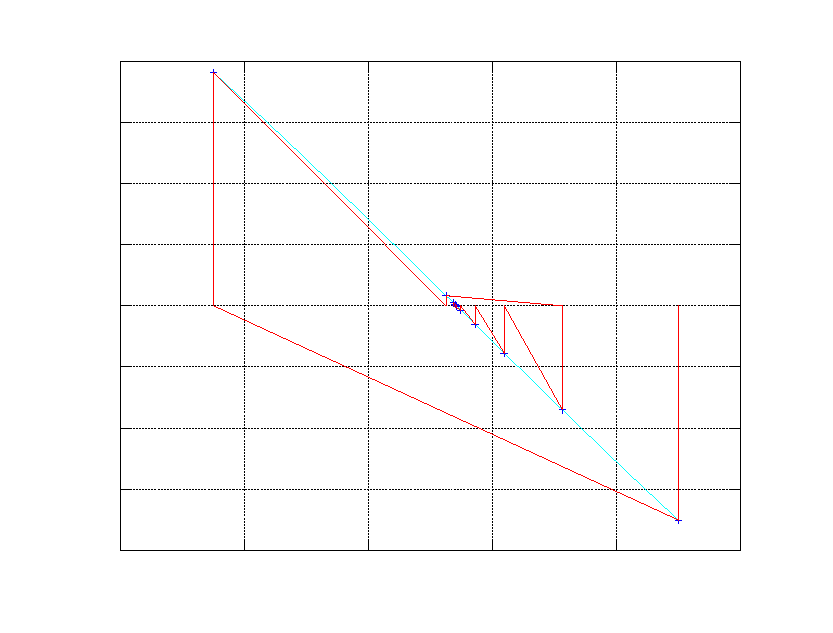
\includegraphics{RadiciEquazione/bisectionPlotOutput}}%
    \gplfronttext
  \end{picture}%
\endgroup

\end{center}

\begin{exercise}
Implementare il metodo di bisezione ed applicarlo alla funzione $\sin(x)$ 
con intervallo iniziale $[-0.1, 7]$, in modo da avere due zeri nell'
intervallo di confidenza, ed una tollerenza $tol_{X} = 10^{-14}$.
\end{exercise}
Per l'implementazione del codice vedere \nameref{sec:bisectionIterativeMethod}.
\begin{lstlisting}
octave:51> [x, i, imax, ascisse] = bisectionMethod('sin', -0.1, 7, e^-14)
x =  6.28318557739258e+00
i =  1.70000000000000e+01
imax =  2.40000000000000e+01
ascisse =
 Columns 1 through 3:
   3.45000000000000e+00   5.22500000000000e+00   6.11250000000000e+00
 Columns 4 through 6:
   6.55625000000000e+00   6.33437500000000e+00   6.22343750000000e+00
 Columns 7 through 9:
   6.27890625000000e+00   6.30664062500000e+00   6.29277343750000e+00
 Columns 10 through 12:
   6.28583984375000e+00   6.28237304687500e+00   6.28410644531250e+00
 Columns 13 through 15:
   6.28323974609375e+00   6.28280639648438e+00   6.28302307128906e+00
 Columns 16 and 17:
   6.28313140869141e+00   6.28318557739258e+00
octave:52> xsin = min(ascisse):0.01:max(ascisse)
octave:53> ysin = feval('sin', xsin)
octave:54> [prepX, prepY] = prepareForPlottingMethodSegments(ascisse, "sin", "")
octave:55> plot(xsin, ysin, "c", ascisse, feval('sin', ascisse), "b+", prepX,
prepY, "r") 
octave:56> print 'bisectionWithTwoRootsPlotOutput.tex' '-dTex' '-S800, 600'
\end{lstlisting}
Si raggiunge la tolleranza richiesta in 17 passi, sette in meno delle iterazioni massime possibili. 
Questo l'output del comando \emph{octave:56}:
\begin{center}
% GNUPLOT: LaTeX picture with Postscript
\begingroup
  \makeatletter
  \providecommand\color[2][]{%
    \GenericError{(gnuplot) \space\space\space\@spaces}{%
      Package color not loaded in conjunction with
      terminal option `colourtext'%
    }{See the gnuplot documentation for explanation.%
    }{Either use 'blacktext' in gnuplot or load the package
      color.sty in LaTeX.}%
    \renewcommand\color[2][]{}%
  }%
  \providecommand\includegraphics[2][]{%
    \GenericError{(gnuplot) \space\space\space\@spaces}{%
      Package graphicx or graphics not loaded%
    }{See the gnuplot documentation for explanation.%
    }{The gnuplot epslatex terminal needs graphicx.sty or graphics.sty.}%
    \renewcommand\includegraphics[2][]{}%
  }%
  \providecommand\rotatebox[2]{#2}%
  \@ifundefined{ifGPcolor}{%
    \newif\ifGPcolor
    \GPcolortrue
  }{}%
  \@ifundefined{ifGPblacktext}{%
    \newif\ifGPblacktext
    \GPblacktexttrue
  }{}%
  % define a \g@addto@macro without @ in the name:
  \let\gplgaddtomacro\g@addto@macro
  % define empty templates for all commands taking text:
  \gdef\gplbacktext{}%
  \gdef\gplfronttext{}%
  \makeatother
  \ifGPblacktext
    % no textcolor at all
    \def\colorrgb#1{}%
    \def\colorgray#1{}%
  \else
    % gray or color?
    \ifGPcolor
      \def\colorrgb#1{\color[rgb]{#1}}%
      \def\colorgray#1{\color[gray]{#1}}%
      \expandafter\def\csname LTw\endcsname{\color{white}}%
      \expandafter\def\csname LTb\endcsname{\color{black}}%
      \expandafter\def\csname LTa\endcsname{\color{black}}%
      \expandafter\def\csname LT0\endcsname{\color[rgb]{1,0,0}}%
      \expandafter\def\csname LT1\endcsname{\color[rgb]{0,1,0}}%
      \expandafter\def\csname LT2\endcsname{\color[rgb]{0,0,1}}%
      \expandafter\def\csname LT3\endcsname{\color[rgb]{1,0,1}}%
      \expandafter\def\csname LT4\endcsname{\color[rgb]{0,1,1}}%
      \expandafter\def\csname LT5\endcsname{\color[rgb]{1,1,0}}%
      \expandafter\def\csname LT6\endcsname{\color[rgb]{0,0,0}}%
      \expandafter\def\csname LT7\endcsname{\color[rgb]{1,0.3,0}}%
      \expandafter\def\csname LT8\endcsname{\color[rgb]{0.5,0.5,0.5}}%
    \else
      % gray
      \def\colorrgb#1{\color{black}}%
      \def\colorgray#1{\color[gray]{#1}}%
      \expandafter\def\csname LTw\endcsname{\color{white}}%
      \expandafter\def\csname LTb\endcsname{\color{black}}%
      \expandafter\def\csname LTa\endcsname{\color{black}}%
      \expandafter\def\csname LT0\endcsname{\color{black}}%
      \expandafter\def\csname LT1\endcsname{\color{black}}%
      \expandafter\def\csname LT2\endcsname{\color{black}}%
      \expandafter\def\csname LT3\endcsname{\color{black}}%
      \expandafter\def\csname LT4\endcsname{\color{black}}%
      \expandafter\def\csname LT5\endcsname{\color{black}}%
      \expandafter\def\csname LT6\endcsname{\color{black}}%
      \expandafter\def\csname LT7\endcsname{\color{black}}%
      \expandafter\def\csname LT8\endcsname{\color{black}}%
    \fi
  \fi
  \setlength{\unitlength}{0.0500bp}%
  \begin{picture}(7680.00,5760.00)%
    \gplgaddtomacro\gplbacktext{%
      \colorrgb{0.00,0.00,0.00}%
      \put(866,634){\makebox(0,0)[r]{\strut{}-1}}%
      \colorrgb{0.00,0.00,0.00}%
      \put(866,1304){\makebox(0,0)[r]{\strut{}-0.8}}%
      \colorrgb{0.00,0.00,0.00}%
      \put(866,1975){\makebox(0,0)[r]{\strut{}-0.6}}%
      \colorrgb{0.00,0.00,0.00}%
      \put(866,2645){\makebox(0,0)[r]{\strut{}-0.4}}%
      \colorrgb{0.00,0.00,0.00}%
      \put(866,3316){\makebox(0,0)[r]{\strut{}-0.2}}%
      \colorrgb{0.00,0.00,0.00}%
      \put(866,3986){\makebox(0,0)[r]{\strut{}0}}%
      \colorrgb{0.00,0.00,0.00}%
      \put(866,4657){\makebox(0,0)[r]{\strut{}0.2}}%
      \colorrgb{0.00,0.00,0.00}%
      \put(866,5327){\makebox(0,0)[r]{\strut{}0.4}}%
      \colorrgb{0.00,0.00,0.00}%
      \put(998,414){\makebox(0,0){\strut{}3}}%
      \colorrgb{0.00,0.00,0.00}%
      \put(1742,414){\makebox(0,0){\strut{}3.5}}%
      \colorrgb{0.00,0.00,0.00}%
      \put(2486,414){\makebox(0,0){\strut{}4}}%
      \colorrgb{0.00,0.00,0.00}%
      \put(3230,414){\makebox(0,0){\strut{}4.5}}%
      \colorrgb{0.00,0.00,0.00}%
      \put(3974,414){\makebox(0,0){\strut{}5}}%
      \colorrgb{0.00,0.00,0.00}%
      \put(4718,414){\makebox(0,0){\strut{}5.5}}%
      \colorrgb{0.00,0.00,0.00}%
      \put(5462,414){\makebox(0,0){\strut{}6}}%
      \colorrgb{0.00,0.00,0.00}%
      \put(6206,414){\makebox(0,0){\strut{}6.5}}%
      \colorrgb{0.00,0.00,0.00}%
      \put(6950,414){\makebox(0,0){\strut{}7}}%
    }%
    \gplgaddtomacro\gplfronttext{%
    }%
    \gplbacktext
    \put(0,0){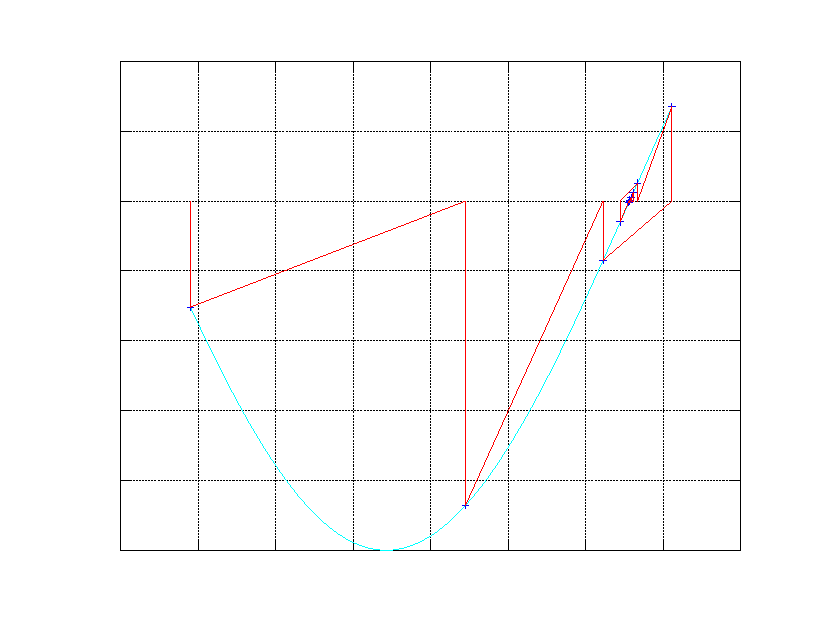
\includegraphics{RadiciEquazione/bisectionWithTwoRootsPlotOutput}}%
    \gplfronttext
  \end{picture}%
\endgroup

\end{center}

Da questo esercizio si vede che il metodo di bisezione converge comunque
ad una radice (in questa applicazione a $2\pi$), anche nel caso in cui
nell'intervallo di confidenza ci sono pi\`u zeri della funzione.





\section{Metodo di Newton}
\label{sec:metodoDiNewton}

\begin{exercise}
Implementare il metodo di newton ed applicarlo alla funzione \emph{singleZero},
con innesco iniziale $x_{0} = 7$, una tollerenza assoluta e relativa
$tol_{X} = rTol_{X} = 10^{-14}$ ed un numero massimo di iterazioni
$i_{max} = 10^{2}$.
\end{exercise}
Per l'implementazione del codice vedere \nameref{sec:newtonIterativeMethod}.
\begin{lstlisting}
octave:112> [x, i, ascisse] = newtonMethod('singleZero','singleZeroDerivative',7, 1e2, 1e-14, 1e-14, 'incrementCriterion') 
x =  3.40512483795333e+00
i =  5.00000000000000e+00
ascisse = [too long to report here]
octave:113> xSingleZero = min(ascisse)-1:0.1:max(ascisse)+1
octave:114> ySingleZero = invokeDelegate('singleZero', xSingleZero)
octave:115> [prepX, prepY] = prepareForPlottingMethodSegments(ascisse, 'invokeDelegate', 'singleZero')
octave:116> plot(xSingleZero, ySingleZero, "c", ascisse, invokeDelegate('singleZero', ascisse), "b+", prepX, prepY, "r")
octave:117> grid
octave:118> print 'newtonPlotOutput.tex' '-dTex' '-S800, 600'
\end{lstlisting}
Si raggiunge la tolleranza richiesta in 5 passi. Questo l'output del comando
\emph{octave:118}:
\begin{center}
% GNUPLOT: LaTeX picture with Postscript
\begingroup
  \makeatletter
  \providecommand\color[2][]{%
    \GenericError{(gnuplot) \space\space\space\@spaces}{%
      Package color not loaded in conjunction with
      terminal option `colourtext'%
    }{See the gnuplot documentation for explanation.%
    }{Either use 'blacktext' in gnuplot or load the package
      color.sty in LaTeX.}%
    \renewcommand\color[2][]{}%
  }%
  \providecommand\includegraphics[2][]{%
    \GenericError{(gnuplot) \space\space\space\@spaces}{%
      Package graphicx or graphics not loaded%
    }{See the gnuplot documentation for explanation.%
    }{The gnuplot epslatex terminal needs graphicx.sty or graphics.sty.}%
    \renewcommand\includegraphics[2][]{}%
  }%
  \providecommand\rotatebox[2]{#2}%
  \@ifundefined{ifGPcolor}{%
    \newif\ifGPcolor
    \GPcolortrue
  }{}%
  \@ifundefined{ifGPblacktext}{%
    \newif\ifGPblacktext
    \GPblacktexttrue
  }{}%
  % define a \g@addto@macro without @ in the name:
  \let\gplgaddtomacro\g@addto@macro
  % define empty templates for all commands taking text:
  \gdef\gplbacktext{}%
  \gdef\gplfronttext{}%
  \makeatother
  \ifGPblacktext
    % no textcolor at all
    \def\colorrgb#1{}%
    \def\colorgray#1{}%
  \else
    % gray or color?
    \ifGPcolor
      \def\colorrgb#1{\color[rgb]{#1}}%
      \def\colorgray#1{\color[gray]{#1}}%
      \expandafter\def\csname LTw\endcsname{\color{white}}%
      \expandafter\def\csname LTb\endcsname{\color{black}}%
      \expandafter\def\csname LTa\endcsname{\color{black}}%
      \expandafter\def\csname LT0\endcsname{\color[rgb]{1,0,0}}%
      \expandafter\def\csname LT1\endcsname{\color[rgb]{0,1,0}}%
      \expandafter\def\csname LT2\endcsname{\color[rgb]{0,0,1}}%
      \expandafter\def\csname LT3\endcsname{\color[rgb]{1,0,1}}%
      \expandafter\def\csname LT4\endcsname{\color[rgb]{0,1,1}}%
      \expandafter\def\csname LT5\endcsname{\color[rgb]{1,1,0}}%
      \expandafter\def\csname LT6\endcsname{\color[rgb]{0,0,0}}%
      \expandafter\def\csname LT7\endcsname{\color[rgb]{1,0.3,0}}%
      \expandafter\def\csname LT8\endcsname{\color[rgb]{0.5,0.5,0.5}}%
    \else
      % gray
      \def\colorrgb#1{\color{black}}%
      \def\colorgray#1{\color[gray]{#1}}%
      \expandafter\def\csname LTw\endcsname{\color{white}}%
      \expandafter\def\csname LTb\endcsname{\color{black}}%
      \expandafter\def\csname LTa\endcsname{\color{black}}%
      \expandafter\def\csname LT0\endcsname{\color{black}}%
      \expandafter\def\csname LT1\endcsname{\color{black}}%
      \expandafter\def\csname LT2\endcsname{\color{black}}%
      \expandafter\def\csname LT3\endcsname{\color{black}}%
      \expandafter\def\csname LT4\endcsname{\color{black}}%
      \expandafter\def\csname LT5\endcsname{\color{black}}%
      \expandafter\def\csname LT6\endcsname{\color{black}}%
      \expandafter\def\csname LT7\endcsname{\color{black}}%
      \expandafter\def\csname LT8\endcsname{\color{black}}%
    \fi
  \fi
  \setlength{\unitlength}{0.0500bp}%
  \begin{picture}(7680.00,5760.00)%
    \gplgaddtomacro\gplbacktext{%
      \colorrgb{0.00,0.00,0.00}%
      \put(866,634){\makebox(0,0)[r]{\strut{}-10}}%
      \colorrgb{0.00,0.00,0.00}%
      \put(866,1304){\makebox(0,0)[r]{\strut{}0}}%
      \colorrgb{0.00,0.00,0.00}%
      \put(866,1975){\makebox(0,0)[r]{\strut{}10}}%
      \colorrgb{0.00,0.00,0.00}%
      \put(866,2645){\makebox(0,0)[r]{\strut{}20}}%
      \colorrgb{0.00,0.00,0.00}%
      \put(866,3316){\makebox(0,0)[r]{\strut{}30}}%
      \colorrgb{0.00,0.00,0.00}%
      \put(866,3986){\makebox(0,0)[r]{\strut{}40}}%
      \colorrgb{0.00,0.00,0.00}%
      \put(866,4657){\makebox(0,0)[r]{\strut{}50}}%
      \colorrgb{0.00,0.00,0.00}%
      \put(866,5327){\makebox(0,0)[r]{\strut{}60}}%
      \colorrgb{0.00,0.00,0.00}%
      \put(998,414){\makebox(0,0){\strut{}2}}%
      \colorrgb{0.00,0.00,0.00}%
      \put(1990,414){\makebox(0,0){\strut{}3}}%
      \colorrgb{0.00,0.00,0.00}%
      \put(2982,414){\makebox(0,0){\strut{}4}}%
      \colorrgb{0.00,0.00,0.00}%
      \put(3974,414){\makebox(0,0){\strut{}5}}%
      \colorrgb{0.00,0.00,0.00}%
      \put(4966,414){\makebox(0,0){\strut{}6}}%
      \colorrgb{0.00,0.00,0.00}%
      \put(5958,414){\makebox(0,0){\strut{}7}}%
      \colorrgb{0.00,0.00,0.00}%
      \put(6950,414){\makebox(0,0){\strut{}8}}%
    }%
    \gplgaddtomacro\gplfronttext{%
    }%
    \gplbacktext
    \put(0,0){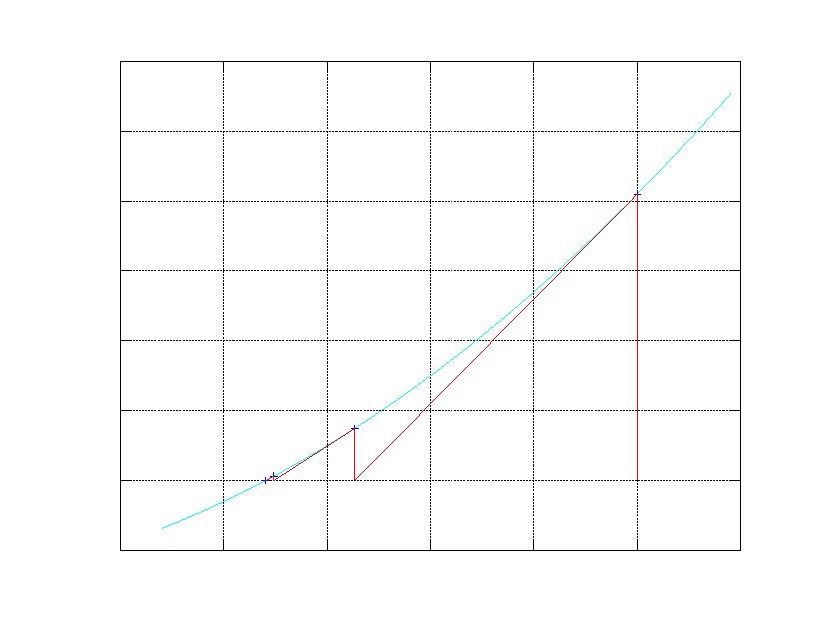
\includegraphics{RadiciEquazione/newton/newtonPlotOutput}}%
    \gplfronttext
  \end{picture}%
\endgroup

\end{center}

\begin{oss}
Per l'applicazione eseguita sopra ho utilizzato il criterio di arresto
\emph{incremento}, il metodo converge, ma posso studiare il condizionamento che
affetta ogni valutazione della precisione richiesta. Questo il codice che
dimostra questo condizionamento, comparando l'applicazione del metodo usando il
criterio di arresto per \emph{residuo}:
\begin{lstlisting}
[x, i, incAscisse, incChecked] = newtonMethod('singleZero','singleZeroDerivative', 7, 1e2, 10^(-14), 10^(-14), 'incrementCriterion');
octave:138> i
i =  5.00000000000000e+00
octave:139> errors = errorMonitor(incAscisse)
errors =
   4.12195121951219e+00   9.88875669244497e+00   8.93522817393261e+01   8.95110152113953e+03   9.18666331414061e+07   7.66765947567831e+15
octave:140> incChecked 
incChecked =
   2.73333333333333e+00   7.83682983682984e-01   7.70978577615202e-02   7.60913136916397e-04   7.41319183816813e-08   8.88178419700125e-16
octave:141> [x, i, resAscisse, resChecked] = newtonMethod('singleZero','singleZeroDerivative', 7, 1e2, 10^(-14), 10^(-14), 'residueCriterion');
octave:142> resChecked 
resChecked =
   2.73333333333333e+00   7.83682983682984e-01   7.70978577615201e-02   7.60913136916414e-04   7.41319183470686e-08   6.82317562092805e-16
octave:143> i
i =  5.00000000000000e+00
\end{lstlisting}
Si osserva che i valori utilizzati nel controllo per il raggiungimento della
precisione richiesta sono uguali tranne l'ultimo, il metodo che usa il criterio
\emph{residueCriterion} \`e pi\`u accurato, in quanto non \`e affetto dalla
cancellazione numerica (per l'ultima coppia di ascisse trovata il fattore di
amplificazione \`e $k = 7.66765947567831e+15$). 

I due metodi utilizzano comunque
lo stesso numero di passi per convergere alla soluzione.
\end{oss}

\begin{oss}
Posso effettuare una nuova comparazione: se chiedo una precisione di $tol_{X}
= 1e-16$, si osserva che il metodo non converge se si utilizza il criterio di 
arresto per \emph{incremento}, mentre converge usando il criterio per
\emph{residuo}. Questo il codice che dimostra quanto detto:
\begin{lstlisting}
octave:5> [x, i]=newtonMethod('singleZero','singleZeroDerivative', 7, 1e2, 10^(-16), 10^(-16),'incrementCriterion');
Il metodo non converge.
octave:6> [x, i]=newtonMethod('singleZero','singleZeroDerivative', 7, 1e2, 10^(-16), 10^(-16),'residueCriterion');
octave:7> i
i =  6
octave:8>
\end{lstlisting}
A parit\`a di numero massimo di passi, il secondo criterio permette al metodo di
convergere.
\end{oss}


\begin{exercise}
Implementare il metodo di newton ed applicarlo alla funzione \emph{functionWithNoRealZero},
con innesco iniziale $x_{0} = 2.5$, una tollerenza assoluta e relativa
$tol_{X} = rTol_{X} = 10^{-14}$ ed un numero massimo di iterazioni
$i_{max} = 7$.
\end{exercise}
Per l'implementazione del codice vedere \nameref{sec:newtonIterativeMethod}.
\begin{lstlisting}
octave:112> [x, i, ascisse] =
newtonMethod('functionWithNoRealZero','functionWithNoRealZeroDerivative', 2.5, 7, 1e-14, 1e-14, 'incrementCriterion') 
Il metodo non converge.
x = -3.18786023393994e+00
i =  7.00000000000000e+00
ascisse = [too long to report here]
octave:113> xNoZero = min(ascisse)-1:0.1:max(ascisse)+1
octave:114> yNoZero = invokeDelegate('functionWithNoRealZero', xNoZero)
octave:115> [prepX, prepY] = prepareForPlottingMethodSegments(ascisse, 'invokeDelegate', 'functionWithNoRealZero')
octave:116> plot(xNoZero, yNoZero, "c", ascisse,invokeDelegate('functionWithNoRealZero', ascisse), "b+", prepX, prepY, "r")
octave:117> grid
octave:118> print 'newtonNoZeroPlotOutput.tex' '-dTex' '-S800, 600'
\end{lstlisting}
Non si raggiunge la convergenza, infatti vengono fatti il massimo possibile
dei passi fissati dal parametro $i_{max}$. Questo l'output del comando \emph{octave:118}:
\begin{center}
% GNUPLOT: LaTeX picture with Postscript
\begingroup
  \makeatletter
  \providecommand\color[2][]{%
    \GenericError{(gnuplot) \space\space\space\@spaces}{%
      Package color not loaded in conjunction with
      terminal option `colourtext'%
    }{See the gnuplot documentation for explanation.%
    }{Either use 'blacktext' in gnuplot or load the package
      color.sty in LaTeX.}%
    \renewcommand\color[2][]{}%
  }%
  \providecommand\includegraphics[2][]{%
    \GenericError{(gnuplot) \space\space\space\@spaces}{%
      Package graphicx or graphics not loaded%
    }{See the gnuplot documentation for explanation.%
    }{The gnuplot epslatex terminal needs graphicx.sty or graphics.sty.}%
    \renewcommand\includegraphics[2][]{}%
  }%
  \providecommand\rotatebox[2]{#2}%
  \@ifundefined{ifGPcolor}{%
    \newif\ifGPcolor
    \GPcolortrue
  }{}%
  \@ifundefined{ifGPblacktext}{%
    \newif\ifGPblacktext
    \GPblacktexttrue
  }{}%
  % define a \g@addto@macro without @ in the name:
  \let\gplgaddtomacro\g@addto@macro
  % define empty templates for all commands taking text:
  \gdef\gplbacktext{}%
  \gdef\gplfronttext{}%
  \makeatother
  \ifGPblacktext
    % no textcolor at all
    \def\colorrgb#1{}%
    \def\colorgray#1{}%
  \else
    % gray or color?
    \ifGPcolor
      \def\colorrgb#1{\color[rgb]{#1}}%
      \def\colorgray#1{\color[gray]{#1}}%
      \expandafter\def\csname LTw\endcsname{\color{white}}%
      \expandafter\def\csname LTb\endcsname{\color{black}}%
      \expandafter\def\csname LTa\endcsname{\color{black}}%
      \expandafter\def\csname LT0\endcsname{\color[rgb]{1,0,0}}%
      \expandafter\def\csname LT1\endcsname{\color[rgb]{0,1,0}}%
      \expandafter\def\csname LT2\endcsname{\color[rgb]{0,0,1}}%
      \expandafter\def\csname LT3\endcsname{\color[rgb]{1,0,1}}%
      \expandafter\def\csname LT4\endcsname{\color[rgb]{0,1,1}}%
      \expandafter\def\csname LT5\endcsname{\color[rgb]{1,1,0}}%
      \expandafter\def\csname LT6\endcsname{\color[rgb]{0,0,0}}%
      \expandafter\def\csname LT7\endcsname{\color[rgb]{1,0.3,0}}%
      \expandafter\def\csname LT8\endcsname{\color[rgb]{0.5,0.5,0.5}}%
    \else
      % gray
      \def\colorrgb#1{\color{black}}%
      \def\colorgray#1{\color[gray]{#1}}%
      \expandafter\def\csname LTw\endcsname{\color{white}}%
      \expandafter\def\csname LTb\endcsname{\color{black}}%
      \expandafter\def\csname LTa\endcsname{\color{black}}%
      \expandafter\def\csname LT0\endcsname{\color{black}}%
      \expandafter\def\csname LT1\endcsname{\color{black}}%
      \expandafter\def\csname LT2\endcsname{\color{black}}%
      \expandafter\def\csname LT3\endcsname{\color{black}}%
      \expandafter\def\csname LT4\endcsname{\color{black}}%
      \expandafter\def\csname LT5\endcsname{\color{black}}%
      \expandafter\def\csname LT6\endcsname{\color{black}}%
      \expandafter\def\csname LT7\endcsname{\color{black}}%
      \expandafter\def\csname LT8\endcsname{\color{black}}%
    \fi
  \fi
  \setlength{\unitlength}{0.0500bp}%
  \begin{picture}(7680.00,5760.00)%
    \gplgaddtomacro\gplbacktext{%
      \colorrgb{0.00,0.00,0.00}%
      \put(866,634){\makebox(0,0)[r]{\strut{}0}}%
      \colorrgb{0.00,0.00,0.00}%
      \put(866,1807){\makebox(0,0)[r]{\strut{}5}}%
      \colorrgb{0.00,0.00,0.00}%
      \put(866,2981){\makebox(0,0)[r]{\strut{}10}}%
      \colorrgb{0.00,0.00,0.00}%
      \put(866,4154){\makebox(0,0)[r]{\strut{}15}}%
      \colorrgb{0.00,0.00,0.00}%
      \put(866,5327){\makebox(0,0)[r]{\strut{}20}}%
      \colorrgb{0.00,0.00,0.00}%
      \put(998,414){\makebox(0,0){\strut{}-6}}%
      \colorrgb{0.00,0.00,0.00}%
      \put(2188,414){\makebox(0,0){\strut{}-4}}%
      \colorrgb{0.00,0.00,0.00}%
      \put(3379,414){\makebox(0,0){\strut{}-2}}%
      \colorrgb{0.00,0.00,0.00}%
      \put(4569,414){\makebox(0,0){\strut{}0}}%
      \colorrgb{0.00,0.00,0.00}%
      \put(5760,414){\makebox(0,0){\strut{}2}}%
      \colorrgb{0.00,0.00,0.00}%
      \put(6950,414){\makebox(0,0){\strut{}4}}%
    }%
    \gplgaddtomacro\gplfronttext{%
    }%
    \gplbacktext
    \put(0,0){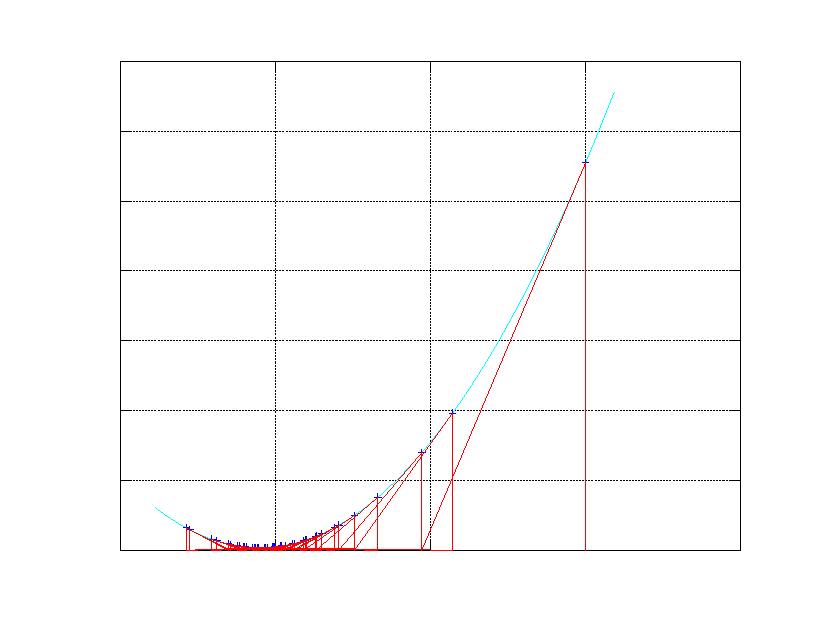
\includegraphics{RadiciEquazione/newton/newtonNoZeroPlotOutput}}%
    \gplfronttext
  \end{picture}%
\endgroup

\end{center}

\begin{exercise}[2.4]
\label{exercise:newtonLoopStartingPoint}
Per il testo dell'esercizio consultare il libro di testo.
\end{exercise}
Per l'implementazione del codice vedere \nameref{sec:newtonIterativeMethod}.

Nel primo caso studio il punto di innesco $x_{0} = 10$:
\begin{lstlisting}
octave:112> [x, i, ascisse] =
newtonMethod('functionNewtonRecursion','functionNewtonRecursionDerivative', 10, 5e1, 1e-14, 1e-14, 'incrementCriterion') 
x =  2.23606797749979e+00
i =  9.00000000000000e+00
ascisse = [too long to report here]
octave:113> xNoZero = min(ascisse)-1:0.1:max(ascisse)+1
octave:114> yNoZero = invokeDelegate('functionNewtonRecursion', xNoZero)
octave:115> [prepX, prepY] = prepareForPlottingMethodSegments(ascisse, 'invokeDelegate', 'functionNewtonRecursion')
octave:116> plot(xNoZero, yNoZero, "c", ascisse,invokeDelegate('functionNewtonRecursion', ascisse), "b+", prepX, prepY, "r")
octave:117> grid
octave:118> print 'newtonRecursivePlotOutput.tex' '-dTex' '-S800, 600'
\end{lstlisting}
Si raggiunge la convergenza con 9 passi. Questo l'output del comando
\emph{octave:118}:
\begin{center}
% GNUPLOT: LaTeX picture with Postscript
\begingroup
  \makeatletter
  \providecommand\color[2][]{%
    \GenericError{(gnuplot) \space\space\space\@spaces}{%
      Package color not loaded in conjunction with
      terminal option `colourtext'%
    }{See the gnuplot documentation for explanation.%
    }{Either use 'blacktext' in gnuplot or load the package
      color.sty in LaTeX.}%
    \renewcommand\color[2][]{}%
  }%
  \providecommand\includegraphics[2][]{%
    \GenericError{(gnuplot) \space\space\space\@spaces}{%
      Package graphicx or graphics not loaded%
    }{See the gnuplot documentation for explanation.%
    }{The gnuplot epslatex terminal needs graphicx.sty or graphics.sty.}%
    \renewcommand\includegraphics[2][]{}%
  }%
  \providecommand\rotatebox[2]{#2}%
  \@ifundefined{ifGPcolor}{%
    \newif\ifGPcolor
    \GPcolortrue
  }{}%
  \@ifundefined{ifGPblacktext}{%
    \newif\ifGPblacktext
    \GPblacktexttrue
  }{}%
  % define a \g@addto@macro without @ in the name:
  \let\gplgaddtomacro\g@addto@macro
  % define empty templates for all commands taking text:
  \gdef\gplbacktext{}%
  \gdef\gplfronttext{}%
  \makeatother
  \ifGPblacktext
    % no textcolor at all
    \def\colorrgb#1{}%
    \def\colorgray#1{}%
  \else
    % gray or color?
    \ifGPcolor
      \def\colorrgb#1{\color[rgb]{#1}}%
      \def\colorgray#1{\color[gray]{#1}}%
      \expandafter\def\csname LTw\endcsname{\color{white}}%
      \expandafter\def\csname LTb\endcsname{\color{black}}%
      \expandafter\def\csname LTa\endcsname{\color{black}}%
      \expandafter\def\csname LT0\endcsname{\color[rgb]{1,0,0}}%
      \expandafter\def\csname LT1\endcsname{\color[rgb]{0,1,0}}%
      \expandafter\def\csname LT2\endcsname{\color[rgb]{0,0,1}}%
      \expandafter\def\csname LT3\endcsname{\color[rgb]{1,0,1}}%
      \expandafter\def\csname LT4\endcsname{\color[rgb]{0,1,1}}%
      \expandafter\def\csname LT5\endcsname{\color[rgb]{1,1,0}}%
      \expandafter\def\csname LT6\endcsname{\color[rgb]{0,0,0}}%
      \expandafter\def\csname LT7\endcsname{\color[rgb]{1,0.3,0}}%
      \expandafter\def\csname LT8\endcsname{\color[rgb]{0.5,0.5,0.5}}%
    \else
      % gray
      \def\colorrgb#1{\color{black}}%
      \def\colorgray#1{\color[gray]{#1}}%
      \expandafter\def\csname LTw\endcsname{\color{white}}%
      \expandafter\def\csname LTb\endcsname{\color{black}}%
      \expandafter\def\csname LTa\endcsname{\color{black}}%
      \expandafter\def\csname LT0\endcsname{\color{black}}%
      \expandafter\def\csname LT1\endcsname{\color{black}}%
      \expandafter\def\csname LT2\endcsname{\color{black}}%
      \expandafter\def\csname LT3\endcsname{\color{black}}%
      \expandafter\def\csname LT4\endcsname{\color{black}}%
      \expandafter\def\csname LT5\endcsname{\color{black}}%
      \expandafter\def\csname LT6\endcsname{\color{black}}%
      \expandafter\def\csname LT7\endcsname{\color{black}}%
      \expandafter\def\csname LT8\endcsname{\color{black}}%
    \fi
  \fi
  \setlength{\unitlength}{0.0500bp}%
  \begin{picture}(7680.00,5760.00)%
    \gplgaddtomacro\gplbacktext{%
      \colorrgb{0.00,0.00,0.00}%
      \put(866,634){\makebox(0,0)[r]{\strut{}-500}}%
      \colorrgb{0.00,0.00,0.00}%
      \put(866,1807){\makebox(0,0)[r]{\strut{}0}}%
      \colorrgb{0.00,0.00,0.00}%
      \put(866,2981){\makebox(0,0)[r]{\strut{}500}}%
      \colorrgb{0.00,0.00,0.00}%
      \put(866,4154){\makebox(0,0)[r]{\strut{}1000}}%
      \colorrgb{0.00,0.00,0.00}%
      \put(866,5327){\makebox(0,0)[r]{\strut{}1500}}%
      \colorrgb{0.00,0.00,0.00}%
      \put(998,414){\makebox(0,0){\strut{}0}}%
      \colorrgb{0.00,0.00,0.00}%
      \put(1990,414){\makebox(0,0){\strut{}2}}%
      \colorrgb{0.00,0.00,0.00}%
      \put(2982,414){\makebox(0,0){\strut{}4}}%
      \colorrgb{0.00,0.00,0.00}%
      \put(3974,414){\makebox(0,0){\strut{}6}}%
      \colorrgb{0.00,0.00,0.00}%
      \put(4966,414){\makebox(0,0){\strut{}8}}%
      \colorrgb{0.00,0.00,0.00}%
      \put(5958,414){\makebox(0,0){\strut{}10}}%
      \colorrgb{0.00,0.00,0.00}%
      \put(6950,414){\makebox(0,0){\strut{}12}}%
    }%
    \gplgaddtomacro\gplfronttext{%
    }%
    \gplbacktext
    \put(0,0){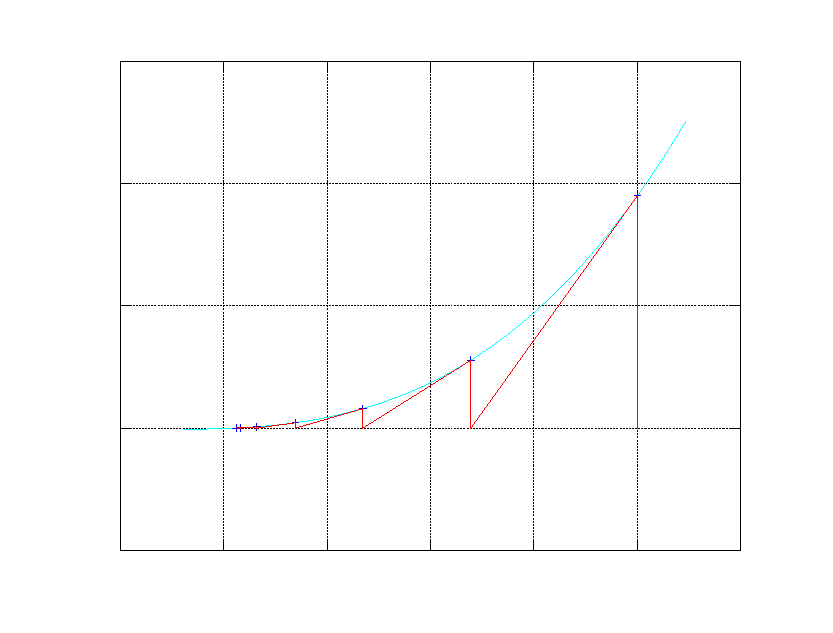
\includegraphics{RadiciEquazione/newton/newtonRecursivePlotOutput}}%
    \gplfronttext
  \end{picture}%
\endgroup

\end{center}

Nel secondo caso studio il punto di innesco $x_{0} = 1$:
\begin{lstlisting}
octave:112> [x, i, ascisse] =
newtonMethod('functionNewtonRecursion','functionNewtonRecursionDerivative', 1, 5e1, 1e-14, 1e-14, 'incrementCriterion') 
Il metodo non converge.
x = -1.00000000000000e+00
i =  5.00000000000000e+01
ascisse = [too long to report here]
octave:113> xNoZero = min(ascisse)-1:0.1:max(ascisse)+1
octave:114> yNoZero = invokeDelegate('functionNewtonRecursion', xNoZero)
octave:115> [prepX, prepY] = prepareForPlottingMethodSegments(ascisse, 'invokeDelegate', 'functionNewtonRecursion')
octave:116> plot(xNoZero, yNoZero, "c", ascisse,invokeDelegate('functionNewtonRecursion', ascisse), "b+", prepX, prepY, "r")
octave:117> grid
octave:118> print 'newtonRecursiveNotConvergencePlotOutput.tex' '-dTex' '-S800,600'
\end{lstlisting}
Il metodo non converge creando una finestra come si vede nel grafico. Questo
l'output del comando \emph{octave:118}:
\begin{center}
% GNUPLOT: LaTeX picture with Postscript
\begingroup
  \makeatletter
  \providecommand\color[2][]{%
    \GenericError{(gnuplot) \space\space\space\@spaces}{%
      Package color not loaded in conjunction with
      terminal option `colourtext'%
    }{See the gnuplot documentation for explanation.%
    }{Either use 'blacktext' in gnuplot or load the package
      color.sty in LaTeX.}%
    \renewcommand\color[2][]{}%
  }%
  \providecommand\includegraphics[2][]{%
    \GenericError{(gnuplot) \space\space\space\@spaces}{%
      Package graphicx or graphics not loaded%
    }{See the gnuplot documentation for explanation.%
    }{The gnuplot epslatex terminal needs graphicx.sty or graphics.sty.}%
    \renewcommand\includegraphics[2][]{}%
  }%
  \providecommand\rotatebox[2]{#2}%
  \@ifundefined{ifGPcolor}{%
    \newif\ifGPcolor
    \GPcolortrue
  }{}%
  \@ifundefined{ifGPblacktext}{%
    \newif\ifGPblacktext
    \GPblacktexttrue
  }{}%
  % define a \g@addto@macro without @ in the name:
  \let\gplgaddtomacro\g@addto@macro
  % define empty templates for all commands taking text:
  \gdef\gplbacktext{}%
  \gdef\gplfronttext{}%
  \makeatother
  \ifGPblacktext
    % no textcolor at all
    \def\colorrgb#1{}%
    \def\colorgray#1{}%
  \else
    % gray or color?
    \ifGPcolor
      \def\colorrgb#1{\color[rgb]{#1}}%
      \def\colorgray#1{\color[gray]{#1}}%
      \expandafter\def\csname LTw\endcsname{\color{white}}%
      \expandafter\def\csname LTb\endcsname{\color{black}}%
      \expandafter\def\csname LTa\endcsname{\color{black}}%
      \expandafter\def\csname LT0\endcsname{\color[rgb]{1,0,0}}%
      \expandafter\def\csname LT1\endcsname{\color[rgb]{0,1,0}}%
      \expandafter\def\csname LT2\endcsname{\color[rgb]{0,0,1}}%
      \expandafter\def\csname LT3\endcsname{\color[rgb]{1,0,1}}%
      \expandafter\def\csname LT4\endcsname{\color[rgb]{0,1,1}}%
      \expandafter\def\csname LT5\endcsname{\color[rgb]{1,1,0}}%
      \expandafter\def\csname LT6\endcsname{\color[rgb]{0,0,0}}%
      \expandafter\def\csname LT7\endcsname{\color[rgb]{1,0.3,0}}%
      \expandafter\def\csname LT8\endcsname{\color[rgb]{0.5,0.5,0.5}}%
    \else
      % gray
      \def\colorrgb#1{\color{black}}%
      \def\colorgray#1{\color[gray]{#1}}%
      \expandafter\def\csname LTw\endcsname{\color{white}}%
      \expandafter\def\csname LTb\endcsname{\color{black}}%
      \expandafter\def\csname LTa\endcsname{\color{black}}%
      \expandafter\def\csname LT0\endcsname{\color{black}}%
      \expandafter\def\csname LT1\endcsname{\color{black}}%
      \expandafter\def\csname LT2\endcsname{\color{black}}%
      \expandafter\def\csname LT3\endcsname{\color{black}}%
      \expandafter\def\csname LT4\endcsname{\color{black}}%
      \expandafter\def\csname LT5\endcsname{\color{black}}%
      \expandafter\def\csname LT6\endcsname{\color{black}}%
      \expandafter\def\csname LT7\endcsname{\color{black}}%
      \expandafter\def\csname LT8\endcsname{\color{black}}%
    \fi
  \fi
  \setlength{\unitlength}{0.0500bp}%
  \begin{picture}(7680.00,5760.00)%
    \gplgaddtomacro\gplbacktext{%
      \colorrgb{0.00,0.00,0.00}%
      \put(866,634){\makebox(0,0)[r]{\strut{}-6}}%
      \colorrgb{0.00,0.00,0.00}%
      \put(866,1416){\makebox(0,0)[r]{\strut{}-4}}%
      \colorrgb{0.00,0.00,0.00}%
      \put(866,2198){\makebox(0,0)[r]{\strut{}-2}}%
      \colorrgb{0.00,0.00,0.00}%
      \put(866,2981){\makebox(0,0)[r]{\strut{}0}}%
      \colorrgb{0.00,0.00,0.00}%
      \put(866,3763){\makebox(0,0)[r]{\strut{}2}}%
      \colorrgb{0.00,0.00,0.00}%
      \put(866,4545){\makebox(0,0)[r]{\strut{}4}}%
      \colorrgb{0.00,0.00,0.00}%
      \put(866,5327){\makebox(0,0)[r]{\strut{}6}}%
      \colorrgb{0.00,0.00,0.00}%
      \put(998,414){\makebox(0,0){\strut{}-2}}%
      \colorrgb{0.00,0.00,0.00}%
      \put(1742,414){\makebox(0,0){\strut{}-1.5}}%
      \colorrgb{0.00,0.00,0.00}%
      \put(2486,414){\makebox(0,0){\strut{}-1}}%
      \colorrgb{0.00,0.00,0.00}%
      \put(3230,414){\makebox(0,0){\strut{}-0.5}}%
      \colorrgb{0.00,0.00,0.00}%
      \put(3974,414){\makebox(0,0){\strut{}0}}%
      \colorrgb{0.00,0.00,0.00}%
      \put(4718,414){\makebox(0,0){\strut{}0.5}}%
      \colorrgb{0.00,0.00,0.00}%
      \put(5462,414){\makebox(0,0){\strut{}1}}%
      \colorrgb{0.00,0.00,0.00}%
      \put(6206,414){\makebox(0,0){\strut{}1.5}}%
      \colorrgb{0.00,0.00,0.00}%
      \put(6950,414){\makebox(0,0){\strut{}2}}%
    }%
    \gplgaddtomacro\gplfronttext{%
    }%
    \gplbacktext
    \put(0,0){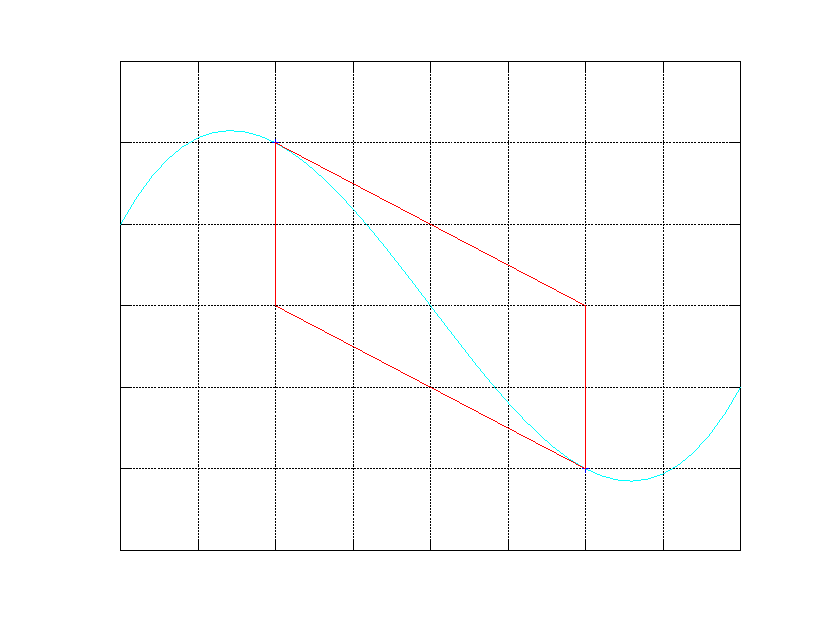
\includegraphics{RadiciEquazione/newton/newtonRecursiveNotConvergencePlotOutput}}%
    \gplfronttext
  \end{picture}%
\endgroup

\end{center}

\chapter{Sistemi lineari}

\section{Esercizi preliminari}

\begin{exercise}[3.2]
\label{exercise:32}
Se $A, B \in \mathbb{R}^{n \times n}$ triangolari inferiori valgono
rispettivamente:
\begin{displaymath}
A + B = C \quad \wedge \quad AB = D
\end{displaymath}
con $C, D \in \mathbb{R}^{n \times n}$ triangolari inferiori.
\end{exercise}
\begin{proof}[Proof of A+B=C]
Per definizione di triangolare inferiore devo dimostrare che $c_{ij} = 0$ se $i
< j$.

Per la definizione dell'operatore $+(,)$ tra matrici ottengo
\begin{displaymath}
c_{ij} = a_{ij} + b_{ij} 
\end{displaymath}
Per ipotesi $A,B$ sono triangolari inferiori, quindi $a_{ij} = b_{ij} = 0$ se
$i < j$, quindi $c_{ij} = 0$ se $i < j$ e questo termina la prova.
\end{proof}

\begin{proof}[Proof of AB=D]
Per definizione di triangolare inferiore devo dimostrare che $c_{ij} = 0$ se $i
< j$.

Per definizione dell'operatore $\cdot(,)$ tra matrici, $d_{ij}$ \`e dato dal
prodotto dell'$i$-esima riga con la $j$-esima colonna, formalmente se $i < j$
\begin{displaymath}
d_{ij} = \left ( \vect{e}_{i}^{T}A \right ) \left ( B \vect{e}_{j} \right) = 
\begin{bmatrix}
a_{i1} \cdots a_{ii} \underbrace{0 \cdots 0}_{n-i}
\end{bmatrix}
\begin{bmatrix}
0 \\
\vdots \\
0 \\
b_{i+1,j}
\\
\vdots \\
b_{nj}
\end{bmatrix} = 0
\end{displaymath}
Svolgendo il prodotto riga-colonna si osserva che le prime $i$ componenti della
colonna annullano le prime $i$ componenti della riga e le ultime $n-i$
componenti della riga annullano le ultime $n-i$ componenti della colonna, quindi
si sommano tutti elementi nulli, per cui
\begin{displaymath}
d_{ij} = \sum_{k = 1}^{n}{a_{ik}b_{kj}} = 0 \quad \text{ se } i < j
\end{displaymath} e questo termina la prova.
\end{proof}

Con argomento simmetrico si dimostra che vale lo stesso asserto se $A,B,C,D \in
\mathbb{R}^{n \times n}$ triangolari superiori.

\begin{exercise}[3.3]
Se $A,B \in \mathbb{R}^{n \times n}$ triangolari inferiori a diagonale unitaria
allora $AB=C$, con $C \in \mathbb{R}^{n \times n}$ triangolare inferiore a
diagonale unitaria.
\end{exercise}
\begin{proof}
$A,B$ sono triangolari inferiori, quindi per l'esercizio \ref{exercise:32},
anche $C$ \`e triangolare inferiore. Rimane da dimostrare che $c_{ii} = 1$ per
$i \in \lbrace 1, \ldots, n\rbrace$.

Posso scrivere $c_{ii}$ come prodotto dell'$i$-esima riga con la $i$-esima
colonna, formalmente se $i \geq j$
\begin{displaymath}
\begin{split}
c_{ii} = \left ( \vect{e}_{i}^{T}A \right ) \left ( B \vect{e}_{i} \right) & =
\begin{bmatrix}
a_{11} \\
\vdots & \ddots \\
a_{i1} & \cdots & a_{ii} \\
\vdots & 		&		& \ddots\\
a_{n1} & \cdots & \cdots &\cdots & a_{nn}
\end{bmatrix} %times 
\begin{bmatrix}
b_{11} \\
\vdots & \ddots \\
b_{i1} & \cdots & b_{ii} \\
\vdots & 		&		& \ddots\\
b_{n1} & \cdots & \cdots &\cdots & b_{nn}
\end{bmatrix} = \\ %split  
&= \begin{bmatrix}
a_{i1} & \cdots & a_{i,i-1} & a_{ii} & 0 & \cdots & 0
\end{bmatrix}
\begin{bmatrix}
0 \\
\vdots \\
0 \\
b_{i,i} \\
b_{i+1,i} \\
\vdots \\
b_{ni}
\end{bmatrix} = \sum_{k = 1}^{n}{a_{in}b_{ni}} = a_{ii}b_{ii} = 1
\end{split}
\end{displaymath}
Svolgendo il prodotto riga-colonna si osserva che le prime $i-1$ componenti
della colonna annullano le prime $i-1$ componenti della riga e le ultime $n-i$
componenti della riga annullano le ultime $n-i$ componenti della colonna, rimane
solo il termine $a_{ii}b_{ii}$, ma per ipotesi $a_{ii}=b_{ii}=1$ perch\`e $A, B$
sono a diagonale unitaria, quindi $c_{ii} = 1$ e questo termina la prova.
\end{proof}

\begin{exercise}[3.4]
\label{exercise:341}
Se $A$ \`e triangolare inferiore allora $A^{-1}$ \`e triangolare inferiore.
\end{exercise}
\begin{proof}
Prova per assurdo.

Le ipotesi di assurdo sono: $A$ triangolare inferiore ed $A^{-1}$ non
triangolare inferiore. 

Per definizione di matrice inversa, chiamo $B = A^{-1}$, $B$ non triangolare
inferiore, vale:
\begin{displaymath}
\begin{bmatrix}
a_{11} \\
\vdots & \ddots \\
a_{i1} & \cdots & a_{ii} \\
\vdots & 		&		& \ddots\\
a_{n1} & \cdots & \cdots &\cdots & a_{nn}
\end{bmatrix} %times 
\begin{bmatrix}
b_{11} & \cdots & \cdots &\cdots & b_{1n} \\
\vdots & \ddots &		&		& \vdots\\
b_{i1} & \cdots & b_{ii} &		& \vdots\\
\vdots & 		&		& \ddots & \vdots\\
b_{n1} & \cdots & \cdots &\cdots & b_{nn}
\end{bmatrix} =
\begin{bmatrix}
1 \\
 & \ddots \\
 & 		& \ddots \\
 & 		&		& \ddots\\
 &  	&  		&		& 1
\end{bmatrix}
\end{displaymath}
Studio come si ottiene la prima riga della matrice identit\`a:
\begin{displaymath}
\vect{e}_{i}^{T} I = 
\begin{bmatrix}
1 & 0 & \ldots & 0
\end{bmatrix} = 
\begin{array}{c}
a_{11}
	\begin{bmatrix}
	b_{11} & \ldots & b_{1n}
	\end{bmatrix} \\
+ 0
	\begin{bmatrix}
	b_{21} & \ldots & b_{2n}
	\end{bmatrix}  \\
\vdots \\
+ 0
	\begin{bmatrix}
	b_{n1} & \ldots & b_{nn}
	\end{bmatrix}
\end{array} =
a_{11}
	\begin{bmatrix}
	b_{11} & \ldots & b_{1n}
	\end{bmatrix} 
\end{displaymath}
Per ipotesi di assurdo $B = A^{-1}$, quindi $b_{11} = \frac{1}{a_{11}}$, e dato
che $A$ \`e triangolare inferiore, allore $a_{11}$ rendendo sensata la
divisione.

Per ipotesi di assurdo $B$ non \`e triangolare inferiore, quindi $\exists k:
b_{1k} \not = 0$ e quindi anche $a_{11}b_{1k} \not = 0$. Ma questo \`e assurdo
perch\`e deve valere 
\begin{displaymath}
\begin{split}
\begin{bmatrix}
1 & 0 & \ldots & 0
\end{bmatrix} \vect{e}_{k} &= 
\begin{bmatrix}
a_{11}b_{11} & \ldots & a_{11}b_{1n}
\end{bmatrix} \vect{e}_{k} \\
0 &= a_{11}b_{1k}
\end{split}
\end{displaymath}
Ma $a_{11}b_{1k} \not = 0$, cado in assurdo, quindi $B=A^{-1}$ deve essere
triangolare inferiore.
\end{proof}

\begin{exercise}[3.4]
Se $A$ \`e triangolare inferiore a diagonale unitaria allora $A^{-1}$ \`e
triangolare inferiore a diagonale unitaria.
\end{exercise}
\begin{proof}
Per ipotesi $A$ \`e triangolare inferiore, per l'esercizio \ref{exercise:341},
anche $A^{-1}$ \`e triangolare inferiore. Rimane da dimostrare che $b_{ii} = 1$
con $b_{ij} \in B = A^{-1}$.

Per definizione di matrice inversa, chiamo $B = A^{-1}$, vale:
\begin{displaymath}
\begin{bmatrix}
1 \\
\vdots & \ddots \\
a_{i1} & \cdots & 1 \\
\vdots & 		&		& \ddots\\
a_{n1} & \cdots & \cdots &\cdots & 1
\end{bmatrix} %times 
\begin{bmatrix}
b_{11} \\
\vdots & \ddots \\
b_{i1} & \cdots & b_{ii} \\
\vdots & 		&		& \ddots \\
b_{n1} & \cdots & \cdots &\cdots & b_{nn}
\end{bmatrix} =
\begin{bmatrix}
1 \\
 & \ddots \\
 & 		& \ddots \\
 & 		&		& \ddots\\
 &  	&  		&		& 1
\end{bmatrix}
\end{displaymath}
Prova per assurdo. Suppongo che $B$ non sia a diagonale unitaria, quindi
$b_{ii} \not = 1$.
Studio come si ottiene la prima riga della matrice identit\`a:
\begin{displaymath}
\vect{e}_{i}^{T} I = 
\begin{bmatrix}
1 & 0 & \ldots & 0
\end{bmatrix} = 
\begin{array}{c}
1
	\begin{bmatrix}
	b_{11} & 0 & \ldots & 0
	\end{bmatrix} \\
+ 0
	\begin{bmatrix}
	b_{21} & b_{22} & 0 & \ldots & 0
	\end{bmatrix}  \\
\vdots \\
+ 0
	\begin{bmatrix}
	b_{n1} & \ldots & b_{nn}
	\end{bmatrix}
\end{array} =
	\begin{bmatrix}
	b_{11} & 0 & \ldots & 0
	\end{bmatrix} 
\end{displaymath}
Affinch\`e sia vera l'uguaglianza deve valere $1 = b_{11}$. Ma questo \`e
assurdo perch\`e per ipotesi di assurdo $b_{11} \not = 1$, quindi $B=A^{-1}$ \`e
triangolare inferiore a diagonale unitaria.
\end{proof}

\begin{exercise}
\label{exercise:triangularMatrixDet}
Se $A$ \`e triangolare allora $\det(A) = a_{11} \cdots a_{nn}$
\end{exercise}
\begin{proof}
Suppongo che $A$ sia triangolare inferiore, lo stesso argomento si dimostra in
modo simmetrico per le matrici triangolari superiori $B$: considerando $B^{T}$
si torna ad una triangolare inferiore e quindi si pu\`o usare questa prova.
Quindi $A$ \`e della forma:
\begin{displaymath}
\begin{bmatrix}
a_{11} \\
\vdots & \ddots \\
a_{i1} & \cdots & a_{ii} \\
\vdots & 		&		& \ddots\\
a_{n1} & \cdots & \cdots &\cdots & a_{nn}
\end{bmatrix}
\end{displaymath}
Calcolo il determinante rispetto alla prima riga:
\begin{displaymath}
\det(A) = a_{11}A_{11} + a_{12}A_{12}\cdots + a_{1n}A_{1n}
\end{displaymath}
Per ipotesi $A$ \`e tringolare inferiore, quindi $a_{ij} = 0$ se $i < j$, quindi
\begin{displaymath}
\det(A) = a_{11}A_{11}
\end{displaymath}
Calcolare $A_{11}$ equivale a calcolare la funzione $\det$ della matrice
$B$ ottenuta da $A$ cancellando la prima riga e la prima colonna:
\begin{displaymath}
B = \begin{bmatrix}
a_{22} \\
\vdots & \ddots \\
a_{i2} & \cdots & a_{ii} \\
\vdots & 		&		& \ddots\\
a_{n2} & \cdots & \cdots &\cdots & a_{nn}
\end{bmatrix}
\end{displaymath}
Ma anche questa matrice \`e una tringolare inferiore, posso riapplicare lo
stesso ragionamento per il calcolo del determinante, ottenendo $\det(B) =
a_{22}B_{11}$, considerare una nuova matrice $C$ ottenuta da $B$ cancellando la
prima riga e la prima colonna. \footnote{si cancella sempre la prima riga e la
prima colonna, in quanto calcolando il determinante di una tringolare inferiore
rispetto alla prima riga, rimane solo il primo elemento $b_{11}, c_{11}, \ldots$
che coincidono rispettivamente con $a_{22}, a_{33}, \ldots$ perch\`e gli
elementi della matrice non vengono modificati nel calcolo del determinante}
Il procedimento ricorsivo si ferma quando si arriva alla sotto-matrice $X$ con
il solo elemento $x_{11} = a_{nn}$ e, per la definizione di $\det$ vale
$\det(a_{nn}) = a_{nn}$. Ricomponenti i pezzi si ottiene $\det(A) = a_{11}
\cdots a_{nn}$ e questo termina la prova.
\end{proof}

\begin{exercise}[3.5, Lemma 3.2]
$A \in \mathbb{R}^{n \times n}$ triangolare. \\
$A$ \`e non singolare sse tutti i suoi
minori principali sono non nulli. 
\end{exercise}
\begin{proof}[Proof of $\Rightarrow$]
Per ipotesi $A$ \`e tringolare e $\det(A) \not = 0$.
Devo dimostrare che $\det(A_{k}) \not = 0, \forall k \in \lbrace 1,\ldots, n
\rbrace$.

Prova per induzione completa su $k$.
\begin{description}
\item[base] per $k = 1$ ottengo $\det{A_{1}} = a_{11}$. Per ipotesi $A$ \`e
triangolare quindi $a_{11} \not = 0$, la base \`e dimostrata.
\item[ipotesi induttiva] suppongo vero $\det(A_{j}) \not = 0, \forall j \in
\lbrace 1,\ldots, k-1 \rbrace$.
\item[passo induttivo] devo dimostrare che $\det(A_{k}) \not = 0$.
Per la definizione della funzione $\det$:
\begin{displaymath}
\det(A) = a_{r1}A_{r1} + \ldots + a_{rn}A_{rn}, \quad \forall r \in {1,\ldots,n}
\end{displaymath}
con $A_{ij} = (-1)^{i+j}M_{ij}(A)$ e $M_{ij}(A)$ restituisce il determinante
della matrice ottenuta non considerando l'$i$-esima riga e la $j$-esima colonna
della matrice $A$ passata come parametro.
\end{description}

Applico la definizione della funzione $\det$ alla sotto-matrice $A_{k}$: per
ipotesi $\det(A) \not = 0$, quindi posso fissare l'indice $r = 1$ della riga
rispetto a cui calcolo il determinante in quanto $\det(A)$ non cambia rispetto
alla riga (e anche alle colonne) rispetto a cui viene calcolato. Ottengo:
\begin{displaymath}
\det(A_{k}) = a_{11}A_{k_{11}} + \ldots + a_{1n}A_{k_{1n}}
\end{displaymath}
Per ipotesi $A$ \`e triangolare quindi $a_{ij} = 0$ per $i < j$, quindi:
\begin{displaymath}
\det(A_{k}) = a_{11}A_{k_{11}}
\end{displaymath}
Ancora usando l'ipotesi che $A$ \`e triangolare, la struttura di triangolare
viene preservata da ogni sua sotto-matrice principale, ovvero $A_{o}$ \`e
tringolare $\forall o \in {1,\ldots,n}$, quindi anche $A_{k}$ \`e tringolare.
Per questo motivo il calcolo di $A_{k_{11}} = (-1)^{1+1}M_{11}(A_{k})$. Dato che
devo calcolare il determinante della nuova matrice $A'$ ottenuta da $A_{k}$ non
considerando la prima riga e la prima colonna, devo calcolare il determinante di
una nuova matrice triangolare. Calcolandolo sempre $\det(A')$ sulla prima riga
ottengo $det(A') = a_{22}A'_{22}$. Ripetendo il ragionamento fino ad arrivare
alla sotto-matrice degenere ad un elemento $A^{k-1} = a_{kk}$, ottengo che: 
\begin{displaymath}
\det(A_{k}) = a_{11}\cdots a_{kk}
\end{displaymath}
Dato che $\det(A) = a_{11} \cdots a_{nn} \not = 0$ per
ipotesi, allora anche $\det(A_{k}) \not = 0$ e questo completa il passo induttivo.
\end{proof}

\begin{proof}[Proof of $\Leftarrow$]
Per ipotesi vale $\det(A_{k}) \not = 0, \forall k \in \lbrace 1, \ldots,
n\rbrace$. Considero la sotto-matrice con $k = n$, quindi $A_{n} = A$.
Applicando la funzione $\det$ ad entrambi i membri, per l'ipotesi si
ottiene l'asserto.
\end{proof}



\begin{exercise}[3.5, Lemma 3.3]
Se $A = LU$ allora 
$\det(A_{k}) = \det(U_{k}), \forall k \in \lbrace 1,\ldots,n \rbrace$
\end{exercise}
\begin{proof}
$\det(A_{k}) = \det(L_{k}U_{k}) = \det(L_{k}) \det(U_{k})$ perch\`e $L_{k}$ e
$U_{k}$ hanno la stessa dimensione. Ma $L_{k}$ \`e tringolare inferiore a
diagonale unitaria per costruzione della \emph{fattorizzazione LU}, quindi
$\det(L_{k}) = 1$, quindi si ottiene l'asserto.
\end{proof}
\section{Before Partial Pivoting}

\begin{exercise}[3.6]
Per il testo dell'esercizio consultare il libro di testo.
\end{exercise}
\begin{proof}
Il numero di operazioni che compio \`e dato da:
\begin{displaymath}
\sum_{i = 1}^{n}{\left( (n-i) + 2(n-i)^{2} \right)} =
\sum_{k = 0}^{n - 1}{\left( k + 2k^{2} \right)} = 
\sum_{k = 0}^{n - 1}{k } + 2\sum_{k = 0}^{n - 1}{k^{2}} 
\end{displaymath}
Con la prima somma si sommano i primi $n-1$ numeri naturali (escludendo lo
zero), per la seconda somma posso applicare il suggerimento del testo 
$\sum_{i = 0}^{n-1}{i^{2}} = \frac{n(n-1)(2n-1)}{6}$, ottengo quindi:
\begin{displaymath}
\begin{split}
\sum_{k = 0}^{n - 1}{k } + 2\sum_{k = 0}^{n - 1}{k^{2}} &= \frac{n(n-1)}{2} +
\frac{2n(n-1)(2n-1)}{6} = n(n-1)\left( \frac{1}{2} + \frac{2n-1}{3}\right ) = \\
&= n(n-1) \frac{4n+1}{6} = (n^{2}-n) \frac{4n+1}{6} = \frac{4n^{3} -3n^{2}-n}{6}
\approx \frac{2}{3}n^{3}
\end{split}
\end{displaymath}
Considerando per l'ultima approssimazione solo il termine di grado massimo.
\end{proof}

\begin{exercise}[3.7, 3.8]
Per i testi degli esercizi consultare il libro di testo.
\end{exercise}
Vedere il codice \nameref{subsection:LUmethod}.

\begin{oss}
Posso vedere il $k$-esimo vettore di Gauss e la relativa matrice elementare come 
delle funzioni:
\begin{displaymath}
\begin{split}
\vect{g}_{k} = g_{k}(\vect{v}) &= \frac{1}{v_{kk}} 
\begin{bmatrix}
0 \\ \vdots \\ 0 \\ v_{k + 1} \\ \vdots \\ v_{n}
\end{bmatrix} \quad , g_{k}: \mathbb{R}^{n} \rightarrow
\mathbb{R}^{n} \\
L = L(\vect{v}) &= I - g_{k}(\vect{v})\vect{e}_{k}^{T}  \quad , L:
\mathbb{R}^{n \times n} \rightarrow \mathbb{R}^{n \times n}
\end{split}
\end{displaymath}
Inoltre al passo $i$-esimo non si modifica la riga $i$: si modificano gli
elementi sotto $a_{ii}$ e tutta la sottomatrice $A(i + 1:n, i + 1:n)$ (scritta
in notazione Octave).
\\\\
L'equazione del testo 3.22 scrive:
\begin{displaymath}
L = I + \vect{g}_{1}\vect{e}_{1}^{T} + \cdots + \vect{g}_{n-1}\vect{e}_{n-1}^{T}
= \begin{bmatrix}
1 \\
g_{21} & 1 \\
\vdots & \ddots		& \ddots \\
g_{n1} & \cdots		&	g_{n,n-1}	& 1
\end{bmatrix}
\end{displaymath}
con 
\begin{displaymath}
g_{ik} = \vect{e}_{i}^{T} g_{k}(A^{(k)}\vect{e}_{k}) = 
\vect{e}_{i}^{T} \left ( \frac{1}{a_{kk}^{(k)}}
\begin{bmatrix}
0 \\ \vdots \\ 0 \\ a_{k + 1, k}^{(k)} \\ \vdots \\ a_{n k}^{(k)}
\end{bmatrix} \right )
\end{displaymath}
\end{oss}

\begin{exercise}[3.9, Lemma 3.4]
Se $A$ \`e diagonale dominante per righe allora lo sono anche tutte le sue
sotto-matrici principali.
\end{exercise}
\begin{proof}
Per ipotesi $A$ \`e diagonale dominante per righe, quindi posso costruire questa 
disuguaglianza:
\begin{displaymath}
|a_{ii}| > \sum_{j = 1 \\j \not = i}^{n}{|a_{ij}|} \geq \sum_{j = 1 \\j \not =
i}^{k}{|a_{ij}|}, \quad k \leq n
\end{displaymath}
con $k$ indice della sotto-matrice di ordine $k$. La disuguaglianza a destra
dimostra l'asserto e la prova \`e terminata.
\end{proof}

\begin{exercise}[3.9, Lemma 3.5]
$A$ \`e diagonale dominante per righe sse $A^{T}$ \`e diagonale dominante per
colonne.
\end{exercise}
\begin{proof}[Proof of $\Rightarrow$]
Per ipotesi $A$ \`e diagonale dominante per righe, ovvero:
\begin{displaymath}
|a_{ii}| > \sum_{j = 1 \\j \not = i}^{n}{|a_{ij}|}
\end{displaymath}
Costruisco la trasposta: se $a_{ij} \in A$ allora $a_{ji} \in A^{T}$. Riscrivo
la definizione precedente:
\begin{displaymath}
|a_{ii}| > \sum_{j = 1 \\j \not = i}^{n}{|a_{ji}|}
\end{displaymath}
Ma questa \`e la definizione di matrice diagonale dominante per colonne e questo
termina la prova.
\end{proof}

\begin{proof}[Proof of $\Leftarrow$]
Con argomento simmetrico si dimostra anche l'implicazione inversa.
\end{proof}

\begin{exercise}[3.10]
Se $A = LDL^{T}$ allora $A$ \`e sdp.
\end{exercise}
\begin{proof}
Devo dimostrare che $A$ soddisfa la definizione sdp:
\begin{itemize}
\item $A = LDL^{T} = (L^{T})^{T}DL^{T} = LDL^{T} = A^{T}$, quindi $A$ \`e
simmetrica.
\item $\forall \vect{x} \in \mathbb{R}^{n}, \vect{x} \not = \vect{0}$ allora
deve valere:
\begin{displaymath}
\vect{x}^{T}A\vect{x} = \vect{x}^{T}LDL^{T}\vect{x} > 0
\end{displaymath}
Costruisco il vettore $\vect{y} = L^{T}\vect{x}$, di conseguenza $\vect{y}^{T}
= \vect{x}^{T}(L^{T})^{T} = \vect{x}^{T}L$. Quindi posso riscrivere
$\vect{y}^{T}D\vect{y} > 0$. Rappresento il prodotto $\vect{y}^{T}(D\vect{y})$:
\begin{displaymath}
\vect{y}^{T}(D\vect{y}) = 
\begin{bmatrix}
y_{1} & \cdots & y_{n}
\end{bmatrix}
\begin{bmatrix}
d_{11} \\
 & d_{22} \\
 & 		& \ddots \\
 & 		&		& \ddots\\
 &  	&  		&		& d_{nn}
\end{bmatrix}
\begin{bmatrix}
y_{1}\\
\vdots \\
y_{n}
\end{bmatrix} = 
\begin{bmatrix}
y_{1} & \cdots & y_{n}
\end{bmatrix}
\begin{bmatrix}
y_{1}d_{11}\\
\vdots \\
y_{n}d_{nn}
\end{bmatrix} =
\sum_{i = 1}^{n}{y_{i}d_{ii}} \geq 0
\end{displaymath} 
In quanto per ipotesi $d_{ii} > 0$. Per avere la somma uguale a 0, si dovrebbe
avere $\vect{y} = \vect{0}$. Ma questo non \`e possibile in quanto $\vect{y}  
= L^{T}\vect{x}$ con $L$ non singolare e $\vect{x} \not = \vect{0}$ per
definizione di sdp. Quindi si ha:
\begin{displaymath}
\sum_{i = 1}^{n}{y_{i}d_{ii}} > 0
\end{displaymath} 
questo \`e quanto richiesta dalla definizione di sdp, quindi $A$ \`e sdp e
questo termina la prova.
\end{itemize}
\end{proof}

\begin{exercise}[3.11]
\label{exercise:311}
Se $A$ \`e non singolare allora $A^{T}A$ e $AA^{T}$ sono sdp.
\end{exercise}
\begin{proof}
Devo verifica che $B = A^{T}A$ sia sdp quindi:
\begin{itemize}
  \item $B = A^{T}A = A^{T}(A^{T})^{T} = A^{T}A = B^{T}$, quindi $B$ \`e
  simmetrica
  \item $\forall \vect{x} \in \mathbb{R}^{n}, \vect{x} \not = \vect{0}$ allora
deve valere:
\begin{displaymath}
\vect{x}^{T}B\vect{x} = \vect{x}^{T}A^{T}A\vect{x} > 0
\end{displaymath}
Costruisco il vettore $\vect{y} = A\vect{x}$, di conseguenza $\vect{y}^{T}
= \vect{x}^{T}A^{T}$. Quindi posso riscrivere
$\vect{y}^{T}\vect{y} > 0$ e rappresento:
\begin{displaymath}
\vect{y}^{T}\vect{y} = 
\begin{bmatrix}
y_{1} & \cdots & y_{n}
\end{bmatrix}
\begin{bmatrix}
y_{1}\\
\vdots \\
y_{n}
\end{bmatrix} =
\sum_{i = 1}^{n}{y_{i}^{2}} \geq 0
\end{displaymath} 
Per avere la somma uguale a 0, si dovrebbe
avere $\vect{y} = \vect{0}$. Ma questo non \`e possibile in quanto $\vect{y}  
= A\vect{x}$ con $A$ non singolare, quindi $A$ non \`e la matrice nulla, e
$\vect{x} \not = \vect{0}$ per definizione di sdp. Quindi si ha:
\begin{displaymath}
\sum_{i = 1}^{n}{y_{i}^{2}} > 0
\end{displaymath} 
questo \`e quanto richiesta dalla definizione di sdp, quindi $B$ \`e sdp.

Dato che ho dimostrato che $B$ \`e simmetrica allora anche $B^{T}$ \`e sdp e
questo termina la prova.
\end{itemize}
\end{proof}

\begin{exercise}[3.12]
Se $A \in \mathbb{R}^{m \times n}$, con $m \geq n = rank(A)$ allora $A^{T}A$ \`e
sdp.
\end{exercise}
\begin{proof}
Devo dimostrare che $B = A^{T}A$ \`e sdp.
\begin{itemize}
  \item $B$ per la prova della simmetria dell'esercizio
  \ref{exercise:311}.
  \item $\forall \vect{x} \in \mathbb{R}^{n}, \vect{x} \not = \vect{0}$ allora
  posso costruire un vettore (come fatto nell'esercizio precedente) $\vect{y} =
  A\vect{x}, \vect{y} \in \mathbb{R}^{m}$ ed il rispettivo $\vect{y}^{T} = 
  \vect{x}^{T}A^{T}, \vect{y}^{T} \in \mathbb{R}^{1 \times m}$ e costruire il 
  prodotto richiesto dalla definizione
  \begin{displaymath}
  	\sum_{i = 1}^{m}{y_{i}^{2}} \geq 0
  \end{displaymath}
  Dato che in $A$ ci sono $m-n$ linearmente dipendenti, allora alcuni termini
  della sommatoria $y_{i}$ possono essere nulli. Ma per le ipotesi, $n =
  rank(A)$, quindi esiste un minore principale $\det(A_{k}) \not = 0$. Per come
  \`e costruito $\vect{y}$ allora $\exists i \in \mathbb{N}: y_{i} \not = 0$
  perch\`e $\det(A_{k}) \not = 0$ per ipotesi e $\vect{x} \not = \vect{0}$ per
  la definizione di sdp. Quindi la somma \`e strettamente positiva e questo
  termina la prova.
\end{itemize}
\end{proof}

\begin{exercise}
Sia $S \in \mathbb{R}^{n \times n}$. Se $\det(S) \not = 0$ allora $A = SS^{T}$
\`e sdp.
\end{exercise}
\begin{proof}
Devo dimostrare che $A$ soddisfa le due richieste della definizione di
matrice sdp.
\begin{itemize}
\item $A = SS^{T} = (S^{T})^{T}S^{T} = SS^{T} = A^{T}$, quindi $A$ \`e
simmetrica.
  \item $\forall \vect{x} \in \mathbb{R}^{n}, \vect{x} \not = \vect{0}$ allora
  \begin{displaymath}
\vect{x}^{T}A\vect{x} = \vect{x}^{T}SS^{T}\vect{x} > 0
\end{displaymath}
Costruisco il vettore $\vect{y} = S^{T}\vect{x}$, di conseguenza $\vect{y}^{T}
= \vect{x}^{T}S$. Quindi posso riscrivere
$\vect{y}^{T}\vect{y} > 0$.
Svolgendo il prodotto riga-colonna vale:
\begin{displaymath}
  	\sum_{i = 1}^{n}{y_{i}^{2}} > 0
  \end{displaymath}
  Questa somma non pu\`o essere zero in quanto per come \`e costruito
  $\vect{y}$, per ipotesi $S$ \`e non singolare e dato che $S = S^{T}$,  anche
  $S^{T}$ \`e non singolare, quindi $S^{T}$ non annulla il prodotto. Rimane da
  controllare il vettore $\vect{x}$, ma per costruzione $\vect{x} \not =
  \vect{0}$,  quindi la somma \`e positiva e questo termina la prova che $A =
  SS^{T}$ \`e sdp.
  \end{itemize}
\end{proof}
\begin{oss}
Posso utilizzare l'asserto del precedente esercizio per costruire una matrice
sdp partendo da una matrice non singolare.
\end{oss}

\begin{exercise}[3.13a]
Se $A \in \mathbb{R}^{n \times n}$ allora $A = \frac{1}{2}(A + A^{T}) +
\frac{1}{2}(A - A^{T}) = A_{s} + A_{a}$
\end{exercise}
\begin{proof}
\begin{displaymath}
\begin{split}
\frac{1}{2}
\left (
\begin{bmatrix}
a_{11} & \cdots & \cdots &\cdots & a_{1n} \\
\vdots & \ddots &		&		& \vdots\\
\vdots &  		& \ddots & 		& \vdots\\
\vdots & 		&		& \ddots & \vdots\\
a_{n1} & \cdots & \cdots &\cdots & a_{nn}
\end{bmatrix} + 
\begin{bmatrix}
a_{11} & \cdots & \cdots &\cdots & a_{n1} \\
\vdots & \ddots &		&		& \vdots\\
\vdots &  		& \ddots & 		& \vdots\\
\vdots & 		&		& \ddots & \vdots\\
a_{1n} & \cdots & \cdots &\cdots & a_{nn}
\end{bmatrix} \right ) = \\
= \frac{1}{2} 
\begin{bmatrix}
2a_{11} & \cdots & \cdots &\cdots & a_{1n} + a_{n1} \\
\vdots & \ddots &		&		& \vdots\\
\vdots &  		& \ddots & 		& \vdots\\
\vdots & 		&		& \ddots & \vdots\\
a_{n1} + a_{1n} & \cdots & \cdots &\cdots & 2a_{nn}
\end{bmatrix} = A^{s}
\end{split}
\end{displaymath}
La matrice $A_{s}$ \`e una matrice simmetrica.

Analogamente per la differenza:
\begin{displaymath}
\begin{split}
\frac{1}{2}
\left (
\begin{bmatrix}
a_{11} & \cdots & \cdots &\cdots & a_{1n} \\
\vdots & \ddots &		&		& \vdots\\
\vdots &  		& \ddots & 		& \vdots\\
\vdots & 		&		& \ddots & \vdots\\
a_{n1} & \cdots & \cdots &\cdots & a_{nn}
\end{bmatrix} - 
\begin{bmatrix}
a_{11} & \cdots & \cdots &\cdots & a_{n1} \\
\vdots & \ddots &		&		& \vdots\\
\vdots &  		& \ddots & 		& \vdots\\
\vdots & 		&		& \ddots & \vdots\\
a_{1n} & \cdots & \cdots &\cdots & a_{nn}
\end{bmatrix} \right ) = \\
= \frac{1}{2} 
\begin{bmatrix}
0 & \cdots & \cdots &\cdots & a_{1n} - a_{n1} \\
\vdots & \ddots &		&		& \vdots\\
\vdots &  		& \ddots & 		& \vdots\\
\vdots & 		&		& \ddots & \vdots\\
a_{n1} - a_{1n}& \cdots & \cdots &\cdots & 0
\end{bmatrix} = A^{a}
\end{split}
\end{displaymath}
Verifico che $A_{s} + A_{a} = A$:
\begin{displaymath}
\begin{split}
A_{s} + A_{a} = 
\frac{1}{2}
\begin{bmatrix}
2a_{11} & \cdots & \cdots &\cdots & a_{1n} + a_{n1} + a_{1n} - a_{n1}\\
\vdots & \ddots &		&		& \vdots\\
\vdots &  		& \ddots & 		& \vdots\\
\vdots & 		&		& \ddots & \vdots\\
a_{n1} + a_{1n} + a_{n1} - a_{1n} & \cdots & \cdots &\cdots & 2a_{nn}
\end{bmatrix} = \\
= \frac{1}{2}
\begin{bmatrix}
2a_{11} & \cdots & \cdots &\cdots & 2a_{1n}\\
\vdots & \ddots &		&		& \vdots\\
\vdots &  		& \ddots & 		& \vdots\\
\vdots & 		&		& \ddots & \vdots\\
2a_{n1}& \cdots & \cdots &\cdots & 2a_{nn}
\end{bmatrix} = 
\begin{bmatrix}
a_{11} & \cdots & \cdots &\cdots & a_{1n} \\
\vdots & \ddots &		&		& \vdots\\
\vdots &  		& \ddots & 		& \vdots\\
\vdots & 		&		& \ddots & \vdots\\
a_{n1} & \cdots & \cdots &\cdots & a_{nn}
\end{bmatrix} = A
\end{split}
\end{displaymath}
In generale vale $a'_{ij} = a_{ij} + a_{ji} + a_{ij} - a_{ji} = 2a_{ij}$.
L'uguaglianza \`e verificata e questo termina la prova.
\end{proof}


\begin{exercise}[3.13b]
Se $A \in \mathbb{R}^{n \times n}$ e $\forall \vect{x} \in \mathbb{R}^{n}$
allora $\vect{x}^{T}A\vect{x} = \vect{x}^{T}A_{s}\vect{x}$
\end{exercise}
\begin{proof}
Per la parte $3.13a$ vale che $A = A_{s} + A_{a}$, quindi posso sostituire ed
applicare la propriet\`a distributiva del prodotto:
\begin{displaymath}
\vect{x}^{T}A\vect{x} = \vect{x}^{T}(A_{s} + A_{a})\vect{x} =
\vect{x}^{T}A_{s}\vect{x} + \vect{x}^{T}A_{a}\vect{x}
\end{displaymath}
Posso ridurre l'argomento che si vuole dimostrare ($\vect{x}^{T}A\vect{x} =
\vect{x}^{T}A_{s}\vect{x}$), considerandolo vero, a dimostrare che
necessariamente deve valere $0 = \vect{x}^{T}A_{a}\vect{x}$.

Per definizione di $A_{a}$ vale $\frac{1}{2}(A - A^{T}) = A_{a}$, che posso
rappresentare:
\begin{displaymath}
\frac{1}{2} 
\begin{bmatrix}
0 & a_{12} - a_{21} & \cdots &\cdots & a_{1n} - a_{n1} \\
a_{21} - a_{12} & 0 &		&		& \vdots\\
\vdots &  		& \ddots & 		& \vdots\\
\vdots & 		&		& \ddots & \vdots\\
a_{n1} - a_{1n}& \cdots & \cdots &\cdots & 0
\end{bmatrix} = A^{a}
\end{displaymath}
Fisso un vettore $\vect{x} \in \mathbb{R}^{n}$ e rappresento il prodotto
$\vect{x}^{T}A_{a}\vect{x}$:
\begin{displaymath}
\begin{bmatrix}
x_{1} & \cdots & x_{n}
\end{bmatrix}
\begin{bmatrix}
0 & a_{12} - a_{21} & \cdots &\cdots & a_{1n} - a_{n1} \\
a_{21} - a_{12} & 0 &		&		& \vdots\\
\vdots &  		& \ddots & 		& \vdots\\
\vdots & 		&		& \ddots & \vdots\\
a_{n1} - a_{1n}& \cdots & \cdots &\cdots & 0
\end{bmatrix} 
\begin{bmatrix}
x_{1} \\ 
\vdots \\ 
\vdots \\
\vdots \\
x_{n}
\end{bmatrix}= 2 A^{a}
\end{displaymath}
Sviluppo il prodotto matrice-vettore colonna:
\begin{displaymath}
\begin{bmatrix}
x_{1} & \cdots & x_{n}
\end{bmatrix}
\begin{bmatrix}
0x_{1} + (a_{12} - a_{21})x_{2} + (a_{13} - a_{31})x_{3} + \cdots + (a_{1n} -
a_{n1})x_{n} \\ 
(a_{21} - a_{12})x_{1} + 0x_{2} + (a_{23} - a_{32})x_{3} + \cdots + (a_{2n} -
a_{n2})x_{n} \\ 
\vdots\\
(a_{n1} - a_{1n})x_{1} + (a_{n2} - a_{2n})x_{2} + (a_{n3} - a_{3n})x_{3} +
\cdots + 0x_{n}
\end{bmatrix} = 2 A^{a}
\end{displaymath}
Sviluppo il prodotto vettore riga-vettore colonna ottenendo uno scalare:
\begin{displaymath}
\begin{array}{c}
0x_{1}x_{1} + (a_{12} - a_{21})x_{2}x_{1} + (a_{13} - a_{31})x_{3}x_{1} + \cdots
+ (a_{1n} - a_{n1})x_{n}x_{1} +\\ 
+ (a_{21} - a_{12})x_{1}x_{2} + 0x_{2}x_{2} + (a_{23} - a_{32})x_{3}x_{2} +
\cdots + (a_{2n} - a_{n2})x_{n}x_{2} + \\ 
\vdots\\
+ (a_{n1} - a_{1n})x_{1}x_{n} + (a_{n2} - a_{2n})x_{2}x_{n} + (a_{n3} -
a_{3n})x_{3}x_{n} + \cdots + 0x_{n}x_{n}
\end{array} = 2 A^{a}
\end{displaymath}
Omettendo gli elementi che contengono i fattori $a x_{i} x_{i} = 0$ ottengo:
\begin{displaymath}
0 = \begin{array}{c}
(a_{12} - a_{21})x_{2}x_{1} + (a_{13} - a_{31})x_{3}x_{1} + \cdots
+ (a_{1n} - a_{n1})x_{n}x_{1} +\\ 
+ (a_{21} - a_{12})x_{1}x_{2} + (a_{23} - a_{32})x_{3}x_{2} +
\cdots + (a_{2n} - a_{n2})x_{n}x_{2} + \\ 
\vdots\\
+ (a_{n1} - a_{1n})x_{1}x_{n} + (a_{n2} - a_{2n})x_{2}x_{n} + (a_{n3} -
a_{3n})x_{3}x_{n} + \cdots + (a_{n,n-1} - a_{n-1,n})x_{n-1}x_{n} 
\end{array} = 2 A^{a}
\end{displaymath}
Ma $(a_{ij} - a_{ji})x_{j}x_{i} = -(a_{ji}-a_{ij})x_{i}x_{j}$ quindi tutti gli
elementi della somma precedente si eliminano a coppie. Per completezza dimostro
che il numero di elementi della precedente somma \`e pari. 

Gli elementi della penultima matrice (comprendendo anche i prodotti nulli) \`e
pari al prodotto cartesiano $n^{2}$, sottraggo gli elementi nulli, ovvero la
diagonale, quindi gli elementi non nulli sono $n^{2} - n$. Devo dimostrare
quindi $n^{2} - n = 2k$, con $k \in \mathbb{N}$. Divido per 2 entrambi i membri
ottenendo $\frac{n(n - 1)}{2} = k$. Il primo membro \`e la somma dei primi $n-1$
numeri naturali, quindi $\sum_{i=1}^{n-1}{i} = k$. Ma dato che l'indice
superiore della somma \`e finito ($n-1 <\infty$) allora la somma ammette un
valore finito $k \in \mathbb{N}$, che \`e quello che si voleva dimostrare.
\end{proof}

\begin{exercise}[3.16, 3.17]
Per i testi degli esercizi consultare il libro di testo.
\end{exercise}
Vedere il codice \nameref{subsection:LDLmethod}.

\begin{exercise}[3.18]
Per i testi degli esercizi consultare il libro di testo.
\end{exercise}
\begin{lstlisting}
octave:43> A = [
> 1 1 1 1
> 1 2 2 2
> 1 2 1 1
> 1 2 1 2];
octave:45> [L,U,xs] = LDLmethod(A, [1;1;1;1])
error: A non sdp.
\end{lstlisting}

\begin{exercise}
Usare le fattorizzazioni $LU, LDL^{T}$ alla matrice:
\begin{displaymath}
\begin{bmatrix}
1 & -1 & 0 & 0 \\
-1 & 2 & -1 & 0 \\
0 & -1 & 2 & -1 \\
0 & 0 & -1 & 2
\end{bmatrix}
\end{displaymath}
\end{exercise}

\begin{lstlisting}
octave:49> A = [1 -1 0 0; -1 2 -1 0; 0 -1 2 -1; 0 0 -1 2]
A =
   1  -1   0   0
  -1   2  -1   0
   0  -1   2  -1
   0   0  -1   2
octave:50> [L,U,xs] = LUmethod(A, [1;1;1;1])
L =
   1   0   0   0
  -1   1   0   0
   0  -1   1   0
   0   0  -1   1
U =
   1  -1   0   0
   0   1  -1   0
   0   0   1  -1
   0   0   0   1
xs =
   10
    9
    7
    4
octave:51> [L,D,xs] = LDLmethod(A, [1;1;1;1])
L =
   1   0   0   0
  -1   1   0   0
   0  -1   1   0
   0   0  -1   1
D =
   1   0   0   0
   0   1   0   0
   0   0   1   0
   0   0   0   1
xs =
   10
    9
    7
    4
\end{lstlisting}

\begin{exercise}[3.19]
$a^{(i)}_{ii} \in A^{(i+1)} \in \mathbb{R}^{n \times n}, \quad a^{(i)}_{ii} \not
= 0, \forall i \in {1, \ldots, n}$ se $\det(A) \not = 0$
\end{exercise}
\begin{proof}
Rappresento la matrice $A^{(i+1)}$:	
\begin{displaymath}
A^{(i+1)} = \begin{bmatrix}
a_{k_{1} 1}^{(1)} & \cdots & \cdots &\cdots &\cdots & a_{k_{1} n}^{(1)} \\
0 & \ddots &		&	 &	& \vdots\\
\vdots &  		& a_{k_{i-1}, i-1}^{(i-1)} & 	\cdots	& \cdots & a_{k_{i-1},
n}^{(i-1)}\\ 
\vdots & 		&	0	&	a_{ii}^{(i)}	& \cdots & a_{in}^{(i)}\\
\vdots & 		& \vdots		& \vdots & &\vdots\\
0	   & \cdots & 0 	& a_{ni}^{(i)} &\cdots & a_{nn}^{(i)}
\end{bmatrix} = \lbrace \text{ ragionando a blocchi } \rbrace =  
\begin{array}{c|c}
A_{i-1} & B \\
\hline
0		& C
\end{array}
\end{displaymath}
Adesso posso applicare la funzione ad entrambi i membri pi\`u esterni
dell'uguaglianza, ottengo quindi 
\begin{displaymath}
\det(A^{i+1}) = \det(A_{i-1})\det(C) -
0\det(B) = \det(A_{i-1})\det(C)
\end{displaymath}
Dato che ho potuto raggiungere il passo $i$-esimo della fattorizzazione, allora
significa che $a_{k_{j} j} \not = 0$, con $j \in \lbrace 1, \ldots, i-1
\rbrace$. Osservo che $A_{i-1}$ \`e tringolare inferiore quindi, per l'esercizio 
\ref{exercise:triangularMatrixDet}, vale $\det(A_{i-1}) = a_{k_{1}1}^{(1)}
\cdots a_{k_{i-1} i-1}^{(i-1)} \not = 0$. Ma per ipotesi $A$ \`e
non singolare quindi vale $\det(A^{i+1}) \not = 0$, in quanto sono state $i$
trasformazioni reversibili (basta considerare le $L^{-1}$), ovvero rendono le
due matrici equivalenti. Per questo si ha necessariamente che $\det(C) \not =
0$, ovvero lo colonne della matrice $C$ sono linearmente indipendenti e quindi
\begin{displaymath}
a_{k_{i}i}^{i} = \max_{k \geq i}{|a_{ki}^{(i)}|} \not = 0
\end{displaymath}
in altre parole la colonna $A^{(i+1)}\vect{e}_{i} \not = \vect{0}$.
\end{proof}


\section{After Partial Pivoting}

\begin{exercise}[3.21, 3.22]
Per i testi degli esercizi consultare il libro di testo.
\end{exercise}
Vedere il codice \nameref{subsection:PALUmethod}.

\begin{exercise}[3.23]
Per il testo dell'esercizio consultare il libro di testo.
\end{exercise}
\begin{itemize}
  \item applicazione al sistema dell'esercizio \ref{exercise:324}: si
osserva che usando il pivoting vengono trovate le soluzioni esatte.
\begin{lstlisting}
octave:25> A
A =
   2.22044604925031e-16   1.00000000000000e+00
   1.00000000000000e+00   0.00000000000000e+00
octave:26> b
b =
   1.00000000000000e+00
   2.50000000000000e-01
octave:27> [L, U, p, unknowns] = PALUmethod(A, b)
L =
   1.00000000000000e+00   0.00000000000000e+00
   2.22044604925031e-16   1.00000000000000e+00
U =
   1.00000000000000e+00   0.00000000000000e+00
   0.00000000000000e+00   1.00000000000000e+00
p =
   2.00000000000000e+00   1.00000000000000e+00
unknowns =
   2.50000000000000e-01
   1.00000000000000e+00
\end{lstlisting}

\item applicazione al primo sistema dell'esercizio \ref{exercise:324}:
\begin{lstlisting}
octave:42> A = [ 
1 0 0 0 0 0 0 0 0 0; 
100 1 0 0 0 0 0 0 0 0; 
0 100 1 0 0 0 0 0 0 0; 
0 0 100 1 0 0 0 0 0 0; 
0 0 0 100 1 0 0 0 0 0; 
0 0 0 0 100 1 0 0 0 0; 
0 0 0 0 0 100 1 0 0 0; 
0 0 0 0 0 0 100 1 0 0; 
0 0 0 0 0 0 0 100 1 0; 
0 0 0 0 0 0 0 0 100 1];
octave:43> x = [1 101*ones(1,9)]';
octave:45> [L, U, p, unknowns] = PALUmethod(A, x);
octave:46> format
octave:47> p
p =
    2    3    4    5    6    7    8    9   10    1
octave:50> format long e
octave:51> unknowns'
ans =
 Columns 1 through 4:
   1.00000000000000e+00   1.00000000000000e+00   9.99999999999925e-01   1.00000000000755e+00
 Columns 5 through 8:
   9.99999999245411e-01   1.00000007545890e+00   9.99992454110141e-01   1.00075458898588e+00
 Columns 9 and 10:
   9.24541101412386e-01   8.54588985876136e+00
\end{lstlisting}

\item applicazione al secondo sistema dell'esercizio \ref{exercise:324}:
\begin{lstlisting}
octave:42> A = [ 
1 0 0 0 0 0 0 0 0 0; 
100 1 0 0 0 0 0 0 0 0; 
0 100 1 0 0 0 0 0 0 0; 
0 0 100 1 0 0 0 0 0 0; 
0 0 0 100 1 0 0 0 0 0; 
0 0 0 0 100 1 0 0 0 0; 
0 0 0 0 0 100 1 0 0 0; 
0 0 0 0 0 0 100 1 0 0; 
0 0 0 0 0 0 0 100 1 0; 
0 0 0 0 0 0 0 0 100 1];
octave:43> x = [1 101*ones(1,9)]';
octave:54> y = .1*x;
octave:55> [L, U, p, unknowns] = PALUmethod(A, y);
octave:56> format
octave:57> p
p =
    2    3    4    5    6    7    8    9   10    1
octave:58> format long e
octave:59> unknowns'
ans =
 Columns 1 through 4:
   1.00000000000000e-01   1.00000000000001e-01   9.99999999998550e-02   1.00000000014504e-01
 Columns 5 through 8:
   9.99999985496383e-02   1.00000145036173e-01   9.99854963826791e-02   1.01450361732092e-01
 Columns 9 and 10:
  -4.50361732092139e-02   1.46036173209214e+01
\end{lstlisting} 
\item applicazione al sistema $B\vect{x} = \vect{f}$:
\begin{lstlisting}
octave:59> format 
octave:60> B = [0 1 1; 1 0 1; 2 3 4]
B =
   0   1   1
   1   0   1
   2   3   4
octave:61> f = [1;0;3];
octave:62> [L, U, p, unknowns] = PALUmethod(B, f);
octave:63> L
L =

   1.00000000000000e+00   0.00000000000000e+00   0.00000000000000e+00
   5.00000000000000e-01   1.00000000000000e+00   0.00000000000000e+00
   0.00000000000000e+00  -6.66666666666667e-01   1.00000000000000e+00

octave:64> U
U =
   2.00000000000000e+00   3.00000000000000e+00   4.00000000000000e+00
   0.00000000000000e+00  -1.50000000000000e+00  -1.00000000000000e+00
   0.00000000000000e+00   0.00000000000000e+00   3.33333333333333e-01
octave:66> p
p =
   3   2   1
octave:67> format long e
octave:68> unknowns 
unknowns =
   0.00000000000000e+00
   1.00000000000000e+00
   0.00000000000000e+00
octave:72> B*unknowns - f
ans =
   0
   0
   0
\end{lstlisting}
\end{itemize}

\begin{exercise}[3.24]
\label{exercise:324}
Per il testo dell'esercizio consultare il libro di testo.
\end{exercise}
\begin{lstlisting}
octave:8> A = [eps 1; 1 0], b = [1; 1/4]
A =
   2.22044604925031e-16   1.00000000000000e+00
   1.00000000000000e+00   0.00000000000000e+00
b =
   1.00000000000000e+00
   2.50000000000000e-01
octave:9> A\b
ans =
   2.50000000000000e-01
   1.00000000000000e+00
octave:10> L = [1 0; 1/eps 1], U = [eps 1; 0 -1/eps]
L =
   1.00000000000000e+00   0.00000000000000e+00
   4.50359962737050e+15   1.00000000000000e+00
U =
   2.22044604925031e-16   1.00000000000000e+00
   0.00000000000000e+00  -4.50359962737050e+15
octave:11> (L*U) - A
ans =
   0.00000000000000e+00   0.00000000000000e+00
   0.00000000000000e+00   0.00000000000000e+00
octave:12> U\(L\b)
ans =
   0.00000000000000e+00
   1.00000000000000e+00
\end{lstlisting}
La riga \emph{octave:9} restituisce la soluzione esatta del sistema, ovvero il
vettore $\vect{x} = \bigl [ \begin{smallmatrix}
.25 \\
1
\end{smallmatrix}\bigr ]$.

La riga \emph{octave:11} dimostra che $A = LU$ quindi $0 = LU - A$, le matrici
di fattorizzazione sono corrette.

La riga \emph{octave:12} dimostra che il metodo di fattorizzazione $LU$ senza
pivoting risulta essere mal condizionato, infatti la prima componente
$\tilde{x}_{1} = 0 \not = .25 = x_{1}$.

\begin{exercise}[3.25]
Per il testo dell'esercizio consultare il libro di testo.
\end{exercise}
Per calcolare $k_{\infty}(A)$ \`e necessario calcolare l'inversa:
\begin{displaymath}
\begin{bmatrix}
1 \\
-100 & 1 \\ 
100^{2} & -100 & 1\\ 
-100^{4} & 100^{2} & -100 & 1\\
\vdots & & & & \ddots \\
-100^{16} & 100^{14} & -100^{12} & \cdots & \cdots &  1
\end{bmatrix} = A^{-1}
\end{displaymath}
Questo l'output del codice:
\begin{lstlisting}
octave:35> cond(A,Inf)
warning: inverse: matrix singular to machine precision, rcond = 9.80198e-21
ans =  1.0202e+20
\end{lstlisting}

\begin{exercise}[3.26]
\label{exercise:326}
Per il testo dell'esercizio consultare il libro di testo.
\end{exercise}
Questo il codice che verifica che i vettori $\vect{x}, \vect{y}$ sono soluzioni
rispettivamente delle equazioni $A\vect{x} = \vect{b}, A\vect{y} = \vect{c}$:
\begin{lstlisting}
octave:41> A
A =

     1     0     0     0     0     0     0     0     0     0
   100     1     0     0     0     0     0     0     0     0
     0   100     1     0     0     0     0     0     0     0
     0     0   100     1     0     0     0     0     0     0
     0     0     0   100     1     0     0     0     0     0
     0     0     0     0   100     1     0     0     0     0
     0     0     0     0     0   100     1     0     0     0
     0     0     0     0     0     0   100     1     0     0
     0     0     0     0     0     0     0   100     1     0
     0     0     0     0     0     0     0     0   100     1

octave:42> b = [1;101;101;101;101;101;101;101;101;101];
octave:43> x = [1;1;1;1;1;1;1;1;1;1];
octave:44> A*x - b
ans =
   0
   0
   0
   0
   0
   0
   0
   0
   0
   0
octave:45> c = .1*b;
octave:46> y = [.1;.1;.1;.1;.1;.1;.1;.1;.1;.1];
octave:47> A*y - c
ans =
   0
   0
   0
   0
   0
   0
   0
   0
   0
   0
\end{lstlisting}
Implemento le istruzioni:
\begin{lstlisting}
octave:50> b = [1 101*ones(1,9)]';
octave:51> x(1) = b(1);
octave:52> for i=2:10, x(i) = b(i) - 100*x(i-1); end
octave:53> x = x(:)
x =
   1
   1
   1
   1
   1
   1
   1
   1
   1
   1
octave:54> c = .1*[1 101*ones(1,9)]';
octave:55> y(1) = c(1);
octave:56> for i=2:10, y(i) = c(i) - 100*y(i-1); end
octave:57> y = y(:)
y =
    0.100000
    0.100000
    0.100000
    0.100000
    0.100000
    0.100000
    0.099986
    0.101407
   -0.040702
   14.170153
octave:62> (y-yexact) ./ yexact  
ans =
     0.00000
     0.00000
    -0.00000
     0.00000
    -0.00000
     0.00000
    -0.00014
     0.01407
    -1.40702
   140.70153
\end{lstlisting}
Si osserva che il vettore $\vect{y}$, soluzione esatta del secondo sistema, non
\`e uguale al vettore approssimato dal secondo set di istruzioni: il comando
\emph{octave:62} calcola il vettore degli errori relativi che si commettono e si
nota che per l'ultima componente si ha un errore molto significativo. Questo \`e
dovuto dal fatto che le componenti del vettore dei termini noti $\vect{c}$ non
\`e possibile rappresentarle correttamente in macchina (0.1 ha rappresentazione
infinita periodica in binario). Questi errori di rappresentazione si sommano
nelle 9 iterazioni che vengono fatte dal ciclo for, risultando significative per
la decima componente.

\begin{exercise}[3.28]
Per il testo dell'esercizio consultare il libro di testo.
\end{exercise}
\label{exercise:exercise328}
\begin{proof}
Si vuole dimostrare:
\begin{displaymath}
\beta = -\frac{v_{1}}{\alpha} = \frac{2}{\hat{\vect{v}}^{T}\hat{\vect{v}}},
\quad
\text{con} \quad \hat{\vect{v}} = \frac{\vect{v}}{v_{1}}
\end{displaymath} 
\begin{itemize}
  \item Verifico la concordanza dei segni:
  \begin{displaymath}
    \frac{2}{\hat{\vect{v}}^{T}\hat{\vect{v}}} > 0
  \end{displaymath}
  $\hat{\vect{v}}^{T}\hat{\vect{v}} > 0$ per definizione di norma euclidea.
  Deve quindi valere:
  \begin{displaymath}
  \frac{v_{1}}{\alpha} < 0
  \end{displaymath}
  posso sostituire $v_{1} = z_{1} - \alpha$ e $\alpha =
  -sign(z_{1})||\vect{z}||_{2}$ e $sign(a) = \left \{ \begin{array}{ll} 1 & if
  \quad a \geq 0 \\ -1 & if \quad a
  < 0 \end{array} \right .$ ottenendo:
  \begin{displaymath}
  \frac{z_{1}}{\alpha} - 1 < 0 \Rightarrow \frac{z_{1}}{\alpha} < 1 \Rightarrow
  \frac{sign(z_{1})|z_{1}|}{-sign(z_{1})||\vect{z}||_{2}} < 1 \Rightarrow
  \frac{|z_{1}|}{||\vect{z}||_{2}} > -1
  \end{displaymath}
  Ma questo \`e vero in quanto $|z_{1}| > 0$ per definizione di $|\cdot|$ e
  $||\vect{z}||_{2} > 0$ per definizione di norma euclidea, quindi
  $\frac{|z_{1}|}{||\vect{z}||_{2}} > 0 > -1$. I segni concordano.
  
  \item dimostro l'uguaglianza dei due membri:
  
  Per il primo membro vale:
  \begin{displaymath}
  	-\frac{v_{1}}{\alpha} = 
  	- \frac{sign(z_{1})|z_{1}| -
  	(-sign(z_{1})||\vect{z}||_{2})}{-sign(z_{1})||\vect{z}||_{2}} = -
  	\frac{sign(z_{1})(|z_{1}| + ||\vect{z}||_{2})}{-sign(z_{1})||\vect{z}||_{2}}
  	= \frac{|z_{1}| + ||\vect{z}||_{2}}{||\vect{z}||_{2}}
  \end{displaymath} 
  Per il secondo membro vale:
  \begin{displaymath}
  \begin{split}   
  	\hat{\vect{v}}^{T}\hat{\vect{v}} &= \frac{\vect{v}^{T}\vect{v}}{v_{1}^{2}} =
  	\frac{(\vect{z}^{T} - \alpha \vect{e}_{i}^{T})(\vect{z} -\alpha
  	\vect{e}_{i})}{v_{1}^{2}} = 
  	\frac{\vect{z}^{T}\vect{z} -\alpha \vect{z}^{T}\vect{e}_{i} - \alpha
  	\vect{e}_{i}^{T}\vect{z}
  	+\alpha^{2}\vect{e}_{i}^{T}\vect{e}_{i}}{v_{1}^{2}} = \\
  	&= \frac{\alpha^{2} -\alpha z_{1} - \alpha
  	z_{1}+\alpha^{2}}{v_{1}^{2}} = \frac{2||\vect{z}||_{2}^{2} -2\alpha
  	z_{1}}{v_{1}^{2}} = \frac{2||\vect{z}||_{2}^{2}
  	-2(-sign(z_{1})||\vect{z}||_{2} sign(z_{1})|z_{1}|)}{v_{1}^{2}} = \\
  	&= \frac{2||\vect{z}||_{2}^{2}
  	+2||\vect{z}||_{2}|z_{1}|}{v_{1}^{2}} =
  	\frac{2||\vect{z}||_{2}(||\vect{z}||_{2} +|z_{1}|)}{v_{1}^{2}}
  \end{split}
  \end{displaymath}
  Ma vale che $v_{1} = z_{1} - \alpha = sign(z_{1}) -
  (-sign(z_{1})||\vect{z}||_{2}) = sign(z_{1})(|z_{1}| + ||\vect{z}||_{2})$, per
  cui vale \\$v_{1}^{2} = (|z_{1}| + ||\vect{z}||_{2})^{2}$, quindi posso
  sostituire e semplificare ottenendo:
  \begin{displaymath}
  	\hat{\vect{v}}^{T}\hat{\vect{v}} = \frac{2||\vect{z}||_{2}}{||\vect{z}||_{2}+|z_{1}|}
  \end{displaymath}
  Posso invertire potendo riscrivere il secondo membro come:
  \begin{displaymath}
  \frac{2}{\hat{\vect{v}}^{T}\hat{\vect{v}}} =
  \frac{||\vect{z}||_{2}+|z_{1}|}{||\vect{z}||_{2}} = -\frac{v_{1}}{\alpha} = \beta 
  \end{displaymath}
  e questo termina la prova.
\end{itemize}
\end{proof}

\begin{exercise}[3.29, 3.30]
Per i testi degli esercizi consultare il libro di testo.
\end{exercise}
Vedere il codice \nameref{subsection:QRmethod}.

\begin{exercise}[3.31]
Per il testo dell'esercizio consultare il libro di testo.
\end{exercise}
Questa l'implementazione:
\begin{lstlisting}
octave:37> A = [3 2 1; 1 2 3; 1 2 1; 2 1 2]
A =
   3   2   1
   1   2   3
   1   2   1
   2   1   2
octave:38> b = [10*ones(1,4)]'
b =
   10
   10
   10
   10
octave:39> [houseHolderVectors, Rhat, R, Q, g1, g2, unknowns, residue] =
QRmethod(A,b) houseHolderVectors =
   1.00000   0.00000   0.00000
   0.14550   1.00000   0.00000
   0.14550   0.40559   1.00000
   0.29099  -0.15589  -0.47436
Rhat =
  -3.87298  -3.09839  -2.84019
   0.00000  -1.84391  -1.73544
   0.00000   0.00000   1.98030
   0.00000   0.00000   0.00000
R =
  -3.87298  -3.09839  -2.84019
   0.00000  -1.84391  -1.73544
   0.00000   0.00000   1.98030
Q =
  -0.77460   0.21693  -0.41586  -0.42426
  -0.25820  -0.65079   0.57429  -0.42426
  -0.25820  -0.65079  -0.43566   0.56569
  -0.51640   0.32540   0.55448   0.56569
g1 =
  -18.0739
   -7.5926
    2.7724
g2 =  2.8284
unknowns =
   1.4000
   2.8000
   1.4000
residue =
   1.2000
   1.2000
  -1.6000
  -1.6000
octave:40> R*unknowns -g1 
ans =
   0.0000e+00
  -8.8818e-16
   0.0000e+00
octave:41> norm(R*unknowns -g1 )^2 + norm(g2 )^2
ans =  8.0000
octave:42> r = Q*Rhat*unknowns - b
r =
   1.2000
   1.2000
  -1.6000
  -1.6000
octave:43> norm(r)^2
ans =  8.0000
octave:44> Q*Rhat
ans =
   3.00000   2.00000   1.00000
   1.00000   2.00000   3.00000
   1.00000   2.00000   1.00000
   2.00000   1.00000   2.00000
octave:45> r/norm(r)
ans =
   0.42426
   0.42426
  -0.56569
  -0.56569
\end{lstlisting}
 
\begin{exercise}[3.32]
Per il testo dell'esercizio consultare il libro di testo.
\end{exercise}
Implemento lanciando la funzione \nameref{subsection:functionExercise332}: 
\begin{lstlisting}
octave:13> [unknowns, givenUnknowns] = functionExercise332(0)
unknowns =
 Columns 1 through 3:
   9.63228005156231e+00   9.96322800515623e+00   9.98161400257811e+00
   6.83859974218842e+00   5.18385997421884e+00   5.09192998710942e+00
 Columns 4 through 6:
   9.99632280051562e+00   9.99816140025781e+00   9.99963228005156e+00
   5.01838599742188e+00   5.00919299871094e+00   5.00183859974219e+00
 Columns 7 and 8:
   9.99981614002578e+00   9.99996322800516e+00
   5.00091929987110e+00   5.00018385997422e+00

givenUnknowns =
 Columns 1 through 3:
   9.63228005156232e+00   9.96322800515623e+00   9.98161400257811e+00
   6.83859974218843e+00   5.18385997421885e+00   5.09192998710943e+00
 Columns 4 through 6:
   9.99632280051562e+00   9.99816140025781e+00   9.99963228005156e+00
   5.01838599742189e+00   5.00919299871094e+00   5.00183859974219e+00
 Columns 7 and 8:
   9.99981614002578e+00   9.99996322800515e+00
   5.00091929987110e+00   5.00018385997422e+00
\end{lstlisting}
Riporto quattro grafici relativi a quattro diversi valori di $gamma$.
I grafici in blu sono relativi alla soluzione calcolata con l'implementazione
\nameref{subsection:QRmethod}, mentre i grafici verdi (a obiettivo) e rossi sono
invece relativi al codice dato nell'esercizio. 
\\\\
$gamma = 10$:
\begin{center}
% GNUPLOT: LaTeX picture with Postscript
\begingroup
  \makeatletter
  \providecommand\color[2][]{%
    \GenericError{(gnuplot) \space\space\space\@spaces}{%
      Package color not loaded in conjunction with
      terminal option `colourtext'%
    }{See the gnuplot documentation for explanation.%
    }{Either use 'blacktext' in gnuplot or load the package
      color.sty in LaTeX.}%
    \renewcommand\color[2][]{}%
  }%
  \providecommand\includegraphics[2][]{%
    \GenericError{(gnuplot) \space\space\space\@spaces}{%
      Package graphicx or graphics not loaded%
    }{See the gnuplot documentation for explanation.%
    }{The gnuplot epslatex terminal needs graphicx.sty or graphics.sty.}%
    \renewcommand\includegraphics[2][]{}%
  }%
  \providecommand\rotatebox[2]{#2}%
  \@ifundefined{ifGPcolor}{%
    \newif\ifGPcolor
    \GPcolortrue
  }{}%
  \@ifundefined{ifGPblacktext}{%
    \newif\ifGPblacktext
    \GPblacktexttrue
  }{}%
  % define a \g@addto@macro without @ in the name:
  \let\gplgaddtomacro\g@addto@macro
  % define empty templates for all commands taking text:
  \gdef\gplbacktext{}%
  \gdef\gplfronttext{}%
  \makeatother
  \ifGPblacktext
    % no textcolor at all
    \def\colorrgb#1{}%
    \def\colorgray#1{}%
  \else
    % gray or color?
    \ifGPcolor
      \def\colorrgb#1{\color[rgb]{#1}}%
      \def\colorgray#1{\color[gray]{#1}}%
      \expandafter\def\csname LTw\endcsname{\color{white}}%
      \expandafter\def\csname LTb\endcsname{\color{black}}%
      \expandafter\def\csname LTa\endcsname{\color{black}}%
      \expandafter\def\csname LT0\endcsname{\color[rgb]{1,0,0}}%
      \expandafter\def\csname LT1\endcsname{\color[rgb]{0,1,0}}%
      \expandafter\def\csname LT2\endcsname{\color[rgb]{0,0,1}}%
      \expandafter\def\csname LT3\endcsname{\color[rgb]{1,0,1}}%
      \expandafter\def\csname LT4\endcsname{\color[rgb]{0,1,1}}%
      \expandafter\def\csname LT5\endcsname{\color[rgb]{1,1,0}}%
      \expandafter\def\csname LT6\endcsname{\color[rgb]{0,0,0}}%
      \expandafter\def\csname LT7\endcsname{\color[rgb]{1,0.3,0}}%
      \expandafter\def\csname LT8\endcsname{\color[rgb]{0.5,0.5,0.5}}%
    \else
      % gray
      \def\colorrgb#1{\color{black}}%
      \def\colorgray#1{\color[gray]{#1}}%
      \expandafter\def\csname LTw\endcsname{\color{white}}%
      \expandafter\def\csname LTb\endcsname{\color{black}}%
      \expandafter\def\csname LTa\endcsname{\color{black}}%
      \expandafter\def\csname LT0\endcsname{\color{black}}%
      \expandafter\def\csname LT1\endcsname{\color{black}}%
      \expandafter\def\csname LT2\endcsname{\color{black}}%
      \expandafter\def\csname LT3\endcsname{\color{black}}%
      \expandafter\def\csname LT4\endcsname{\color{black}}%
      \expandafter\def\csname LT5\endcsname{\color{black}}%
      \expandafter\def\csname LT6\endcsname{\color{black}}%
      \expandafter\def\csname LT7\endcsname{\color{black}}%
      \expandafter\def\csname LT8\endcsname{\color{black}}%
    \fi
  \fi
  \setlength{\unitlength}{0.0500bp}%
  \begin{picture}(7680.00,5760.00)%
    \gplgaddtomacro\gplbacktext{%
      \colorrgb{0.00,0.00,0.00}%
      \put(866,634){\makebox(0,0)[r]{\strut{}-20}}%
      \colorrgb{0.00,0.00,0.00}%
      \put(866,1304){\makebox(0,0)[r]{\strut{}0}}%
      \colorrgb{0.00,0.00,0.00}%
      \put(866,1975){\makebox(0,0)[r]{\strut{}20}}%
      \colorrgb{0.00,0.00,0.00}%
      \put(866,2645){\makebox(0,0)[r]{\strut{}40}}%
      \colorrgb{0.00,0.00,0.00}%
      \put(866,3316){\makebox(0,0)[r]{\strut{}60}}%
      \colorrgb{0.00,0.00,0.00}%
      \put(866,3986){\makebox(0,0)[r]{\strut{}80}}%
      \colorrgb{0.00,0.00,0.00}%
      \put(866,4657){\makebox(0,0)[r]{\strut{}100}}%
      \colorrgb{0.00,0.00,0.00}%
      \put(866,5327){\makebox(0,0)[r]{\strut{}120}}%
      \colorrgb{0.00,0.00,0.00}%
      \put(1494,414){\makebox(0,0){\strut{}0}}%
      \colorrgb{0.00,0.00,0.00}%
      \put(2486,414){\makebox(0,0){\strut{}2}}%
      \colorrgb{0.00,0.00,0.00}%
      \put(3478,414){\makebox(0,0){\strut{}4}}%
      \colorrgb{0.00,0.00,0.00}%
      \put(4470,414){\makebox(0,0){\strut{}6}}%
      \colorrgb{0.00,0.00,0.00}%
      \put(5462,414){\makebox(0,0){\strut{}8}}%
      \colorrgb{0.00,0.00,0.00}%
      \put(6454,414){\makebox(0,0){\strut{}10}}%
    }%
    \gplgaddtomacro\gplfronttext{%
    }%
    \gplbacktext
    \put(0,0){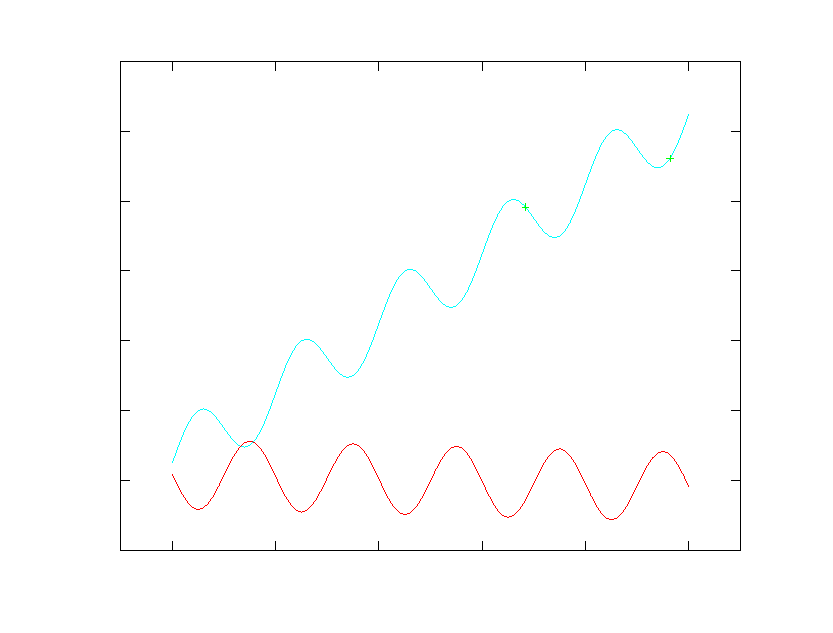
\includegraphics{SistemiLineari/exer332gamma10}}%
    \gplfronttext
  \end{picture}%
\endgroup

\end{center}
$gamma = 5e-1$: 
\begin{center}
% GNUPLOT: LaTeX picture with Postscript
\begingroup
  \makeatletter
  \providecommand\color[2][]{%
    \GenericError{(gnuplot) \space\space\space\@spaces}{%
      Package color not loaded in conjunction with
      terminal option `colourtext'%
    }{See the gnuplot documentation for explanation.%
    }{Either use 'blacktext' in gnuplot or load the package
      color.sty in LaTeX.}%
    \renewcommand\color[2][]{}%
  }%
  \providecommand\includegraphics[2][]{%
    \GenericError{(gnuplot) \space\space\space\@spaces}{%
      Package graphicx or graphics not loaded%
    }{See the gnuplot documentation for explanation.%
    }{The gnuplot epslatex terminal needs graphicx.sty or graphics.sty.}%
    \renewcommand\includegraphics[2][]{}%
  }%
  \providecommand\rotatebox[2]{#2}%
  \@ifundefined{ifGPcolor}{%
    \newif\ifGPcolor
    \GPcolortrue
  }{}%
  \@ifundefined{ifGPblacktext}{%
    \newif\ifGPblacktext
    \GPblacktexttrue
  }{}%
  % define a \g@addto@macro without @ in the name:
  \let\gplgaddtomacro\g@addto@macro
  % define empty templates for all commands taking text:
  \gdef\gplbacktext{}%
  \gdef\gplfronttext{}%
  \makeatother
  \ifGPblacktext
    % no textcolor at all
    \def\colorrgb#1{}%
    \def\colorgray#1{}%
  \else
    % gray or color?
    \ifGPcolor
      \def\colorrgb#1{\color[rgb]{#1}}%
      \def\colorgray#1{\color[gray]{#1}}%
      \expandafter\def\csname LTw\endcsname{\color{white}}%
      \expandafter\def\csname LTb\endcsname{\color{black}}%
      \expandafter\def\csname LTa\endcsname{\color{black}}%
      \expandafter\def\csname LT0\endcsname{\color[rgb]{1,0,0}}%
      \expandafter\def\csname LT1\endcsname{\color[rgb]{0,1,0}}%
      \expandafter\def\csname LT2\endcsname{\color[rgb]{0,0,1}}%
      \expandafter\def\csname LT3\endcsname{\color[rgb]{1,0,1}}%
      \expandafter\def\csname LT4\endcsname{\color[rgb]{0,1,1}}%
      \expandafter\def\csname LT5\endcsname{\color[rgb]{1,1,0}}%
      \expandafter\def\csname LT6\endcsname{\color[rgb]{0,0,0}}%
      \expandafter\def\csname LT7\endcsname{\color[rgb]{1,0.3,0}}%
      \expandafter\def\csname LT8\endcsname{\color[rgb]{0.5,0.5,0.5}}%
    \else
      % gray
      \def\colorrgb#1{\color{black}}%
      \def\colorgray#1{\color[gray]{#1}}%
      \expandafter\def\csname LTw\endcsname{\color{white}}%
      \expandafter\def\csname LTb\endcsname{\color{black}}%
      \expandafter\def\csname LTa\endcsname{\color{black}}%
      \expandafter\def\csname LT0\endcsname{\color{black}}%
      \expandafter\def\csname LT1\endcsname{\color{black}}%
      \expandafter\def\csname LT2\endcsname{\color{black}}%
      \expandafter\def\csname LT3\endcsname{\color{black}}%
      \expandafter\def\csname LT4\endcsname{\color{black}}%
      \expandafter\def\csname LT5\endcsname{\color{black}}%
      \expandafter\def\csname LT6\endcsname{\color{black}}%
      \expandafter\def\csname LT7\endcsname{\color{black}}%
      \expandafter\def\csname LT8\endcsname{\color{black}}%
    \fi
  \fi
  \setlength{\unitlength}{0.0500bp}%
  \begin{picture}(7680.00,5760.00)%
    \gplgaddtomacro\gplbacktext{%
      \colorrgb{0.00,0.00,0.00}%
      \put(866,634){\makebox(0,0)[r]{\strut{}-20}}%
      \colorrgb{0.00,0.00,0.00}%
      \put(866,1304){\makebox(0,0)[r]{\strut{}0}}%
      \colorrgb{0.00,0.00,0.00}%
      \put(866,1975){\makebox(0,0)[r]{\strut{}20}}%
      \colorrgb{0.00,0.00,0.00}%
      \put(866,2645){\makebox(0,0)[r]{\strut{}40}}%
      \colorrgb{0.00,0.00,0.00}%
      \put(866,3316){\makebox(0,0)[r]{\strut{}60}}%
      \colorrgb{0.00,0.00,0.00}%
      \put(866,3986){\makebox(0,0)[r]{\strut{}80}}%
      \colorrgb{0.00,0.00,0.00}%
      \put(866,4657){\makebox(0,0)[r]{\strut{}100}}%
      \colorrgb{0.00,0.00,0.00}%
      \put(866,5327){\makebox(0,0)[r]{\strut{}120}}%
      \colorrgb{0.00,0.00,0.00}%
      \put(1494,414){\makebox(0,0){\strut{}0}}%
      \colorrgb{0.00,0.00,0.00}%
      \put(2486,414){\makebox(0,0){\strut{}2}}%
      \colorrgb{0.00,0.00,0.00}%
      \put(3478,414){\makebox(0,0){\strut{}4}}%
      \colorrgb{0.00,0.00,0.00}%
      \put(4470,414){\makebox(0,0){\strut{}6}}%
      \colorrgb{0.00,0.00,0.00}%
      \put(5462,414){\makebox(0,0){\strut{}8}}%
      \colorrgb{0.00,0.00,0.00}%
      \put(6454,414){\makebox(0,0){\strut{}10}}%
    }%
    \gplgaddtomacro\gplfronttext{%
    }%
    \gplbacktext
    \put(0,0){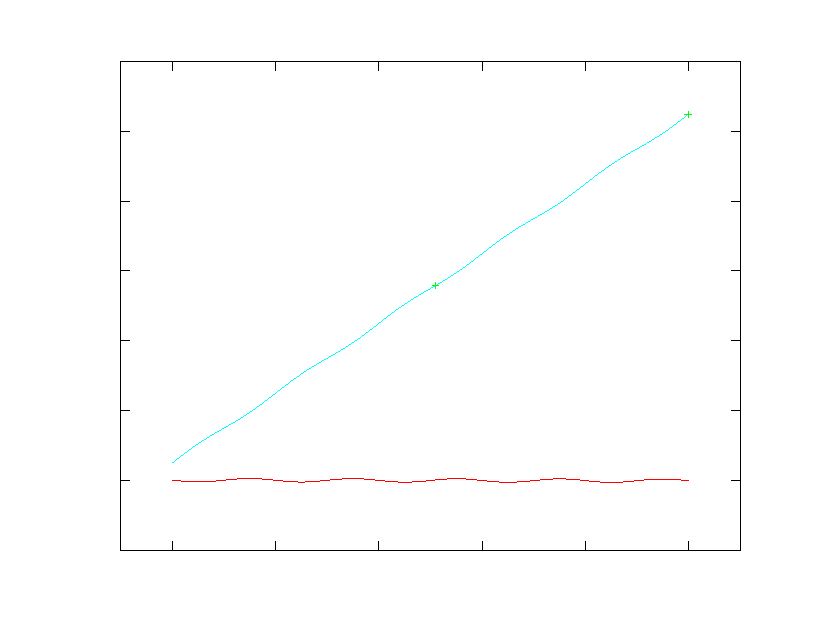
\includegraphics{SistemiLineari/exer332gamma5e-1}}%
    \gplfronttext
  \end{picture}%
\endgroup

\end{center}
$gamma = 1e-1$:
\begin{center}
% GNUPLOT: LaTeX picture with Postscript
\begingroup
  \makeatletter
  \providecommand\color[2][]{%
    \GenericError{(gnuplot) \space\space\space\@spaces}{%
      Package color not loaded in conjunction with
      terminal option `colourtext'%
    }{See the gnuplot documentation for explanation.%
    }{Either use 'blacktext' in gnuplot or load the package
      color.sty in LaTeX.}%
    \renewcommand\color[2][]{}%
  }%
  \providecommand\includegraphics[2][]{%
    \GenericError{(gnuplot) \space\space\space\@spaces}{%
      Package graphicx or graphics not loaded%
    }{See the gnuplot documentation for explanation.%
    }{The gnuplot epslatex terminal needs graphicx.sty or graphics.sty.}%
    \renewcommand\includegraphics[2][]{}%
  }%
  \providecommand\rotatebox[2]{#2}%
  \@ifundefined{ifGPcolor}{%
    \newif\ifGPcolor
    \GPcolortrue
  }{}%
  \@ifundefined{ifGPblacktext}{%
    \newif\ifGPblacktext
    \GPblacktexttrue
  }{}%
  % define a \g@addto@macro without @ in the name:
  \let\gplgaddtomacro\g@addto@macro
  % define empty templates for all commands taking text:
  \gdef\gplbacktext{}%
  \gdef\gplfronttext{}%
  \makeatother
  \ifGPblacktext
    % no textcolor at all
    \def\colorrgb#1{}%
    \def\colorgray#1{}%
  \else
    % gray or color?
    \ifGPcolor
      \def\colorrgb#1{\color[rgb]{#1}}%
      \def\colorgray#1{\color[gray]{#1}}%
      \expandafter\def\csname LTw\endcsname{\color{white}}%
      \expandafter\def\csname LTb\endcsname{\color{black}}%
      \expandafter\def\csname LTa\endcsname{\color{black}}%
      \expandafter\def\csname LT0\endcsname{\color[rgb]{1,0,0}}%
      \expandafter\def\csname LT1\endcsname{\color[rgb]{0,1,0}}%
      \expandafter\def\csname LT2\endcsname{\color[rgb]{0,0,1}}%
      \expandafter\def\csname LT3\endcsname{\color[rgb]{1,0,1}}%
      \expandafter\def\csname LT4\endcsname{\color[rgb]{0,1,1}}%
      \expandafter\def\csname LT5\endcsname{\color[rgb]{1,1,0}}%
      \expandafter\def\csname LT6\endcsname{\color[rgb]{0,0,0}}%
      \expandafter\def\csname LT7\endcsname{\color[rgb]{1,0.3,0}}%
      \expandafter\def\csname LT8\endcsname{\color[rgb]{0.5,0.5,0.5}}%
    \else
      % gray
      \def\colorrgb#1{\color{black}}%
      \def\colorgray#1{\color[gray]{#1}}%
      \expandafter\def\csname LTw\endcsname{\color{white}}%
      \expandafter\def\csname LTb\endcsname{\color{black}}%
      \expandafter\def\csname LTa\endcsname{\color{black}}%
      \expandafter\def\csname LT0\endcsname{\color{black}}%
      \expandafter\def\csname LT1\endcsname{\color{black}}%
      \expandafter\def\csname LT2\endcsname{\color{black}}%
      \expandafter\def\csname LT3\endcsname{\color{black}}%
      \expandafter\def\csname LT4\endcsname{\color{black}}%
      \expandafter\def\csname LT5\endcsname{\color{black}}%
      \expandafter\def\csname LT6\endcsname{\color{black}}%
      \expandafter\def\csname LT7\endcsname{\color{black}}%
      \expandafter\def\csname LT8\endcsname{\color{black}}%
    \fi
  \fi
  \setlength{\unitlength}{0.0500bp}%
  \begin{picture}(7680.00,5760.00)%
    \gplgaddtomacro\gplbacktext{%
      \colorrgb{0.00,0.00,0.00}%
      \put(866,634){\makebox(0,0)[r]{\strut{}-20}}%
      \colorrgb{0.00,0.00,0.00}%
      \put(866,1304){\makebox(0,0)[r]{\strut{}0}}%
      \colorrgb{0.00,0.00,0.00}%
      \put(866,1975){\makebox(0,0)[r]{\strut{}20}}%
      \colorrgb{0.00,0.00,0.00}%
      \put(866,2645){\makebox(0,0)[r]{\strut{}40}}%
      \colorrgb{0.00,0.00,0.00}%
      \put(866,3316){\makebox(0,0)[r]{\strut{}60}}%
      \colorrgb{0.00,0.00,0.00}%
      \put(866,3986){\makebox(0,0)[r]{\strut{}80}}%
      \colorrgb{0.00,0.00,0.00}%
      \put(866,4657){\makebox(0,0)[r]{\strut{}100}}%
      \colorrgb{0.00,0.00,0.00}%
      \put(866,5327){\makebox(0,0)[r]{\strut{}120}}%
      \colorrgb{0.00,0.00,0.00}%
      \put(1494,414){\makebox(0,0){\strut{}0}}%
      \colorrgb{0.00,0.00,0.00}%
      \put(2486,414){\makebox(0,0){\strut{}2}}%
      \colorrgb{0.00,0.00,0.00}%
      \put(3478,414){\makebox(0,0){\strut{}4}}%
      \colorrgb{0.00,0.00,0.00}%
      \put(4470,414){\makebox(0,0){\strut{}6}}%
      \colorrgb{0.00,0.00,0.00}%
      \put(5462,414){\makebox(0,0){\strut{}8}}%
      \colorrgb{0.00,0.00,0.00}%
      \put(6454,414){\makebox(0,0){\strut{}10}}%
    }%
    \gplgaddtomacro\gplfronttext{%
    }%
    \gplbacktext
    \put(0,0){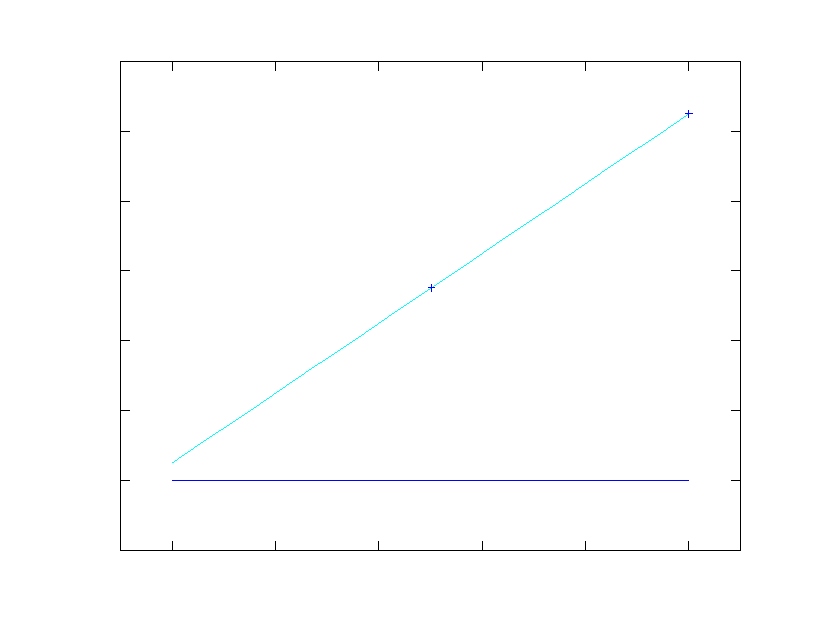
\includegraphics{SistemiLineari/exer332gammae-1}}%
    \gplfronttext
  \end{picture}%
\endgroup

\end{center}
$gamma = 1e-3$:
\begin{center}
% GNUPLOT: LaTeX picture with Postscript
\begingroup
  \makeatletter
  \providecommand\color[2][]{%
    \GenericError{(gnuplot) \space\space\space\@spaces}{%
      Package color not loaded in conjunction with
      terminal option `colourtext'%
    }{See the gnuplot documentation for explanation.%
    }{Either use 'blacktext' in gnuplot or load the package
      color.sty in LaTeX.}%
    \renewcommand\color[2][]{}%
  }%
  \providecommand\includegraphics[2][]{%
    \GenericError{(gnuplot) \space\space\space\@spaces}{%
      Package graphicx or graphics not loaded%
    }{See the gnuplot documentation for explanation.%
    }{The gnuplot epslatex terminal needs graphicx.sty or graphics.sty.}%
    \renewcommand\includegraphics[2][]{}%
  }%
  \providecommand\rotatebox[2]{#2}%
  \@ifundefined{ifGPcolor}{%
    \newif\ifGPcolor
    \GPcolortrue
  }{}%
  \@ifundefined{ifGPblacktext}{%
    \newif\ifGPblacktext
    \GPblacktexttrue
  }{}%
  % define a \g@addto@macro without @ in the name:
  \let\gplgaddtomacro\g@addto@macro
  % define empty templates for all commands taking text:
  \gdef\gplbacktext{}%
  \gdef\gplfronttext{}%
  \makeatother
  \ifGPblacktext
    % no textcolor at all
    \def\colorrgb#1{}%
    \def\colorgray#1{}%
  \else
    % gray or color?
    \ifGPcolor
      \def\colorrgb#1{\color[rgb]{#1}}%
      \def\colorgray#1{\color[gray]{#1}}%
      \expandafter\def\csname LTw\endcsname{\color{white}}%
      \expandafter\def\csname LTb\endcsname{\color{black}}%
      \expandafter\def\csname LTa\endcsname{\color{black}}%
      \expandafter\def\csname LT0\endcsname{\color[rgb]{1,0,0}}%
      \expandafter\def\csname LT1\endcsname{\color[rgb]{0,1,0}}%
      \expandafter\def\csname LT2\endcsname{\color[rgb]{0,0,1}}%
      \expandafter\def\csname LT3\endcsname{\color[rgb]{1,0,1}}%
      \expandafter\def\csname LT4\endcsname{\color[rgb]{0,1,1}}%
      \expandafter\def\csname LT5\endcsname{\color[rgb]{1,1,0}}%
      \expandafter\def\csname LT6\endcsname{\color[rgb]{0,0,0}}%
      \expandafter\def\csname LT7\endcsname{\color[rgb]{1,0.3,0}}%
      \expandafter\def\csname LT8\endcsname{\color[rgb]{0.5,0.5,0.5}}%
    \else
      % gray
      \def\colorrgb#1{\color{black}}%
      \def\colorgray#1{\color[gray]{#1}}%
      \expandafter\def\csname LTw\endcsname{\color{white}}%
      \expandafter\def\csname LTb\endcsname{\color{black}}%
      \expandafter\def\csname LTa\endcsname{\color{black}}%
      \expandafter\def\csname LT0\endcsname{\color{black}}%
      \expandafter\def\csname LT1\endcsname{\color{black}}%
      \expandafter\def\csname LT2\endcsname{\color{black}}%
      \expandafter\def\csname LT3\endcsname{\color{black}}%
      \expandafter\def\csname LT4\endcsname{\color{black}}%
      \expandafter\def\csname LT5\endcsname{\color{black}}%
      \expandafter\def\csname LT6\endcsname{\color{black}}%
      \expandafter\def\csname LT7\endcsname{\color{black}}%
      \expandafter\def\csname LT8\endcsname{\color{black}}%
    \fi
  \fi
  \setlength{\unitlength}{0.0500bp}%
  \begin{picture}(7680.00,5760.00)%
    \gplgaddtomacro\gplbacktext{%
      \colorrgb{0.00,0.00,0.00}%
      \put(866,634){\makebox(0,0)[r]{\strut{}-20}}%
      \colorrgb{0.00,0.00,0.00}%
      \put(866,1304){\makebox(0,0)[r]{\strut{}0}}%
      \colorrgb{0.00,0.00,0.00}%
      \put(866,1975){\makebox(0,0)[r]{\strut{}20}}%
      \colorrgb{0.00,0.00,0.00}%
      \put(866,2645){\makebox(0,0)[r]{\strut{}40}}%
      \colorrgb{0.00,0.00,0.00}%
      \put(866,3316){\makebox(0,0)[r]{\strut{}60}}%
      \colorrgb{0.00,0.00,0.00}%
      \put(866,3986){\makebox(0,0)[r]{\strut{}80}}%
      \colorrgb{0.00,0.00,0.00}%
      \put(866,4657){\makebox(0,0)[r]{\strut{}100}}%
      \colorrgb{0.00,0.00,0.00}%
      \put(866,5327){\makebox(0,0)[r]{\strut{}120}}%
      \colorrgb{0.00,0.00,0.00}%
      \put(1494,414){\makebox(0,0){\strut{}0}}%
      \colorrgb{0.00,0.00,0.00}%
      \put(2486,414){\makebox(0,0){\strut{}2}}%
      \colorrgb{0.00,0.00,0.00}%
      \put(3478,414){\makebox(0,0){\strut{}4}}%
      \colorrgb{0.00,0.00,0.00}%
      \put(4470,414){\makebox(0,0){\strut{}6}}%
      \colorrgb{0.00,0.00,0.00}%
      \put(5462,414){\makebox(0,0){\strut{}8}}%
      \colorrgb{0.00,0.00,0.00}%
      \put(6454,414){\makebox(0,0){\strut{}10}}%
    }%
    \gplgaddtomacro\gplfronttext{%
    }%
    \gplbacktext
    \put(0,0){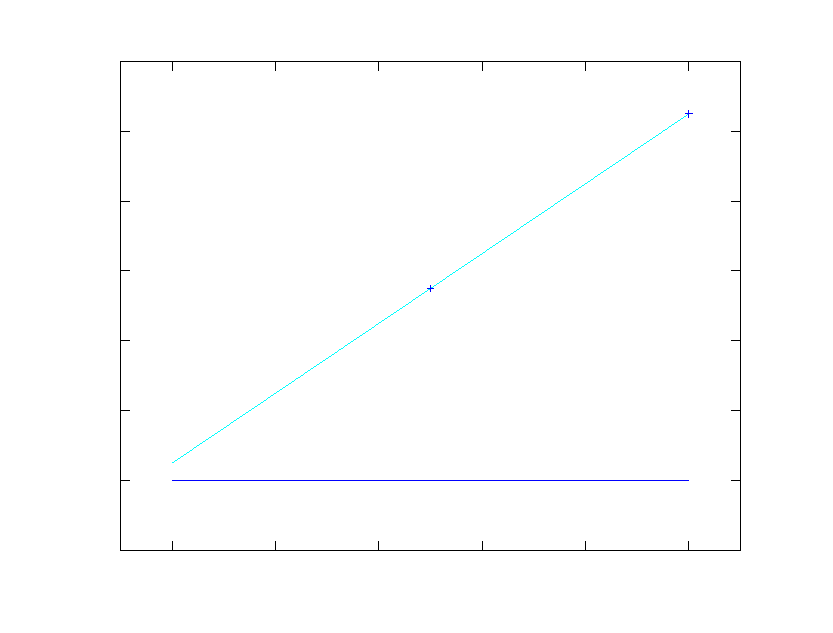
\includegraphics{SistemiLineari/exer332gammae-3}}%
    \gplfronttext
  \end{picture}%
\endgroup

\end{center}
Per $gamma \rightarrow \infty$ si raggiunge la soluzione ottima del sistema
$A\vect{x} = \vect{b} + \vect{r}$ con $\vect{r} = \vect{0}$.


\chapter{Sorgenti Octave}

\section{Metodo iterativo}
\label{sec:iterativeMethodToSQRT2}
\lstinputlisting{listings/chapterOne/iterative.m}

\section{Utility functions}
\subsection{invokeDelegate}
\lstinputlisting{listings/chapterTwo/invokeDelegate.m}

\subsection{prepareForPlottingMethodSegments}
\lstinputlisting{listings/chapterTwo/prepareForPlottingMethodSegments.m}

\section{Metodo di bisezione}
\label{sec:bisectionIterativeMethod}
\lstinputlisting{listings/chapterTwo/bisectionMethod.m}

\section{Metodo di Newton}
\label{sec:newtonIterativeMethod}
Questa implementazione utilizza il criterio di arresto esposto nell'
\emph{Osservazione 2.3} nel caso di radici semplici.

Una osservazione sul numero di passi effettuati: per la mia implementazione
vale $i = length(ascisse) + 2$ in quanto nel ciclo \emph{while} colleziono
$length(ascisse)$ valori, pi\`u uno per il valore di innesco iniziale, pi\`u uno
per l'ultimo valore appena usciti dal ciclo \emph{while}.
\lstinputlisting{listings/chapterTwo/newtonMethod.m}

\section{Varianti del metodo di Newton}

\subsection{Molteplicit\`a dello zero nota}
\label{subsec:newtonMethodMultKnown}
Questa implementazione utilizza il criterio di arresto esposto nell'
\emph{Osservazione 2.3} nel caso di radici semplici.
\lstinputlisting{listings/chapterTwo/newtonMethodMoltKnown.m}

\subsection{Molteplicit\`a dello zero nota con criterio di arresto lineare}
\label{subsec:newtonMethodMultKnownLinearStopCriteria}
Questa implementazione utilizza il criterio di arresto esposto nell'
\emph{Osservazione 2.3} nel caso di radici multiple, ovvero il criterio di
arresto sar\`a dato da:
\begin{displaymath}
	|x_{i+1} - x_{i}| \leq \frac{1-c}{c}tol_{X}
\end{displaymath}
Ricavo in modo dinamico la costante $c$, usando le tre iterate pi\`u recenti:
\begin{displaymath}
	c \approx \frac{|x_{i} - x_{i-1}|}{|x_{i-1} - x_{i-2}|}
\end{displaymath}
Posso usare questa approssimazione in quanto $m > 1$ per ipotesi del problema,
quindi per il \emph{Teorema 2.2}, il metodo di Newton converge linearmente verso zeri
multipli, 
condizione necessaria per applicare questo criterio di arresto.
\lstinputlisting{listings/chapterTwo/newtonMethodMoltKnownLinearCriteria.m}

\section{Fattorizzazioni}
\subsection{triangularSystemSolver}
\lstinputlisting{listings/chapterThree/triangularSystemSolver.m}

\subsection{normalizationEngine}
\lstinputlisting{listings/chapterThree/normalizationEngine.m}

\subsection{LUmethod}
\label{subsection:LUmethod}
\lstinputlisting{listings/chapterThree/LUmethod.m}

\subsection{LDLmethod}
\label{subsection:LDLmethod}
\lstinputlisting{listings/chapterThree/LDLmethod.m}

\subsection{PALUmethod}
\label{subsection:PALUmethod}
\lstinputlisting{listings/chapterThree/PALUmethod.m}

\subsection{QRmethod}
\label{subsection:QRmethod}
\begin{oss}[Sull'uso e costruzione delle matrici di eliminazione $H$]
Durante il metodo non vengono create e sviluppate in modo esplicito le matrici
di eliminazione $H^{i}$ per effettuare i prodotti $H^{i}\vect{v}$: vengono
invece costruite in modo implicito, ovvero la computazione che viene effettuata
dal metodo \`e direttamente la trasformazione ortogonale 
\begin{displaymath}
H\vect{v} \rightarrow \vect{v} -
\frac{2}{\vect{z}^{T}\vect{z}}\vect{z}(\vect{z}^{T}\vect{v})
\end{displaymath}
\end{oss}

\begin{oss}[Sul costo del prodotto scalare]
Dati due vettori $\vect{a}, \vect{b} \in \mathbb{R}^{k}$, il prodotto scalare
costa $2k - 1$ operazioni, di cui $k$ per i prodotti $\forall i \in
\{1, \ldots , k \} [a_{i}b_{i}]$, e $k-1$ somme dei $k$ prodotti.
\end{oss}

\begin{oss}[Idee alla base del metodo]
Queste sono le idee alla base del metodo:
\begin{itemize}
  \item $H(\beta \vect{z}) = H(\vect{z}), \forall \beta \in \mathbb{R}$, ovvero
  la matrice di eliminazione non varia per multipli del vettore caratteristico
  $\vect{z}$ di Householder (permette quindi di scegliere $\beta$ in modo
  da avere il vettore caratteristico con una struttura particolare, $z_{1} =
  1$).
  
  \item la seguente ugualianza permette di evitare il calcolo del prodotto
  scalare, risparmiando $2m$ operazioni:
  	\begin{displaymath}
  		-\frac{z_{1}}{\alpha} =
  		\frac{2}{\vect{z}^{T}\vect{z}}
  	\end{displaymath}
  vedi esercizio \ref{exercise:exercise328}.
  
  \item $v_{1} = A(i, i) - \alpha$ con $\alpha A(i, i) < 0$, permette di
  evitare il fenomeno della cancellazione numerica.
\end{itemize}
\end{oss}

\begin{oss}[Sulla struttura delle matrici di eliminazione $H^{i}$]

\end{oss}

\begin{oss}[Forma matriciale del passo di aggiornamento]
\begin{displaymath}
\begin{bmatrix}
a_{i+1, j}^{(i+1)} \\
\vdots \\
a_{m, j}^{(i+1)}
\end{bmatrix} = 
\begin{bmatrix}
a_{i+1, j}^{(i)} \\
\vdots \\
a_{m, j}^{(i)}
\end{bmatrix} - \frac{2}{(\vect{z}^{(i+1)})^{T} \vect{z}^{(i+1)}} %times
\left ( (\vect{z}^{(i+1)})^{T} \begin{bmatrix}
a_{i+1, j}^{(i+1)} \\
\vdots \\
a_{m, j}^{(i+1)} 
\end{bmatrix} \right )\vect{z}^{(i+1)}
\end{displaymath}
\end{oss}

\lstinputlisting{listings/chapterThree/QRmethod.m}

\subsection{functionExercise332}
\label{subsection:functionExercise332}
\lstinputlisting{listings/chapterThree/functionExercise332.m}

\chapter*{Help di Octave}

\section{Helps for \nameref{sec:metodoDiBisezione} section}

Riporto qui alcune righe di help per le funzioni che verranno utilizzate 
pi\`u spesso in questo capitolo:

\begin{lstlisting}
octave:1> help poly
`poly' is a function from the file /usr/share/octave/3.2.3/m/polynomial/poly.m

 -- Function File:  poly (A)
     If A is a square N-by-N matrix, `poly (A)' is the row vector of
     the coefficients of `det (z * eye (N) - a)', the characteristic
     polynomial of A.  As an example we can use this to find the
     eigenvalues of A as the roots of `poly (A)'.
          roots(poly(eye(3)))
          => 1.00000 - 0.00000i
          => 1.00000 + 0.00000i
     In real-life examples you should, however, use the `eig' function
     for computing eigenvalues.

     If X is a vector, `poly (X)' is a vector of coefficients of the
     polynomial whose roots are the elements of X.  That is, of C is a
     polynomial, then the elements of `D = roots (poly (C))' are
     contained in C.  The vectors C and D are, however, not equal due
     to sorting and numerical errors.

     See also: eig, roots
\end{lstlisting}

\begin{lstlisting}
octave:1> help ones
`ones' is a built-in function

 -- Built-in Function:  ones (X)
 -- Built-in Function:  ones (N, M)
 -- Built-in Function:  ones (N, M, K, ...)
 -- Built-in Function:  ones (..., CLASS)
     Return a matrix or N-dimensional array whose elements are all 1.
     The arguments are handled the same as the arguments for `eye'.

     If you need to create a matrix whose values are all the same, you
     should use an expression like

          val_matrix = val * ones (n, m)
\end{lstlisting}

\begin{lstlisting}
octave:1> help polyval
`polyval' is a function from the file /usr/share/octave/3.2.3/m/polynomial/polyval.m

 -- Function File: Y = polyval (P, X)
 -- Function File: Y = polyval (P, X, [], MU)
     Evaluate the polynomial at of the specified values for X.  When MU
     is present evaluate the polynomial for (X-MU(1))/MU(2).  If X is a
     vector or matrix, the polynomial is evaluated for each of the
     elements of X.

 -- Function File: [Y, DY] = polyval (P, X, S)
 -- Function File: [Y, DY] = polyval (P, X, S, MU)
     In addition to evaluating the polynomial, the second output
     represents the prediction interval, Y +/- DY, which contains at
     least 50% of the future predictions.  To calculate the prediction
     interval, the structured variable S, originating form `polyfit',
     must be present.

     See also: polyfit, polyvalm, poly, roots, conv, deconv, residue,
     filter, polyderiv, polyinteg
\end{lstlisting}

\begin{lstlisting}
octave:14> help ceil
`ceil' is a built-in function

 -- Mapping Function:  ceil (X)
     Return the smallest integer not less than X.  This is equivalent to
     rounding towards positive infinity.  If X is complex, return `ceil
     (real (X)) + ceil (imag (X)) * I'.
          ceil ([-2.7, 2.7])
            =>  -2   3

     See also: floor, round, fix
\end{lstlisting}


\end{document} 
